\documentclass{article}

% If needed:
% \PassOptionsToPackage{numbers,compress}{natbib}

% NeurIPS 2026 style
\PassOptionsToPackage{numbers,compress}{natbib}

\usepackage{neurips_2026}
% For camera-ready, use:
% \usepackage[final]{neurips_2026}
% For preprint, use:
% \usepackage[preprint]{neurips_2026}

\usepackage[utf8]{inputenc}
\usepackage[T1]{fontenc}

\usepackage[dvipsnames]{xcolor}
\definecolor{Bleu}{RGB}{0,0,204}

\usepackage{hyperref}
\hypersetup{
  colorlinks=true,
  citecolor=Bleu,
  linkcolor=Bleu,
  urlcolor=Bleu,
  hypertexnames=false
}

\usepackage{amsmath,amssymb,amsthm,mathtools}
\usepackage{amsfonts}
\usepackage{bbm}
\usepackage{algorithm}
\usepackage{algorithmic}
\usepackage{booktabs}
\usepackage{wrapfig}
\usepackage{graphicx}
\usepackage{enumitem}
\usepackage{microtype}
\usepackage{multirow}
\usepackage{url}
\usepackage{cleveref}
\usepackage{nicefrac}

% Theorem environments
\newtheorem{theorem}{Theorem}
\newtheorem{lemma}{Lemma}
\newtheorem{assumption}{Assumption}
\newtheorem{proposition}{Proposition}
\newtheorem{corollary}{Corollary}

% Macros
\newcommand{\E}{\mathbb{E}}
\newcommand{\Var}{\mathrm{Var}}
\newcommand{\Prob}{\mathbb{P}}
\newcommand{\1}{\mathbbm{1}}
\newcommand{\calS}{\mathcal{S}}
\newcommand{\calA}{\mathcal{A}}
\newcommand{\calD}{\mathcal{D}}
\newcommand{\calP}{\mathcal{P}}
\newcommand{\calV}{\mathcal{V}}
\newcommand{\KL}{\mathrm{KL}}
\newcommand{\R}{\mathbb{R}}
\newcommand{\norm}[1]{\left\lVert #1 \right\rVert}
\newcommand{\ip}[2]{\left\langle #1,\,#2 \right\rangle}
\newcommand{\softmax}{\mathrm{softmax}}
\newcommand{\ubar}[1]{\underline{#1}}
\newcommand{\obar}[1]{\overline{#1}}
\newcommand{\Ind}{\mathbbm{1}}
\newcommand{\wh}{\widehat}
\newcommand{\wt}{\widetilde}
\newcommand{\ustar}{u^\star}

\newcommand{\todo}[1]{\textcolor{red}{[TODO: #1]}}

\title{Modular Inverse Reinforcement Learning\\via Policy Estimation and \(Q\)-Evaluation}

\author{%
  Lars van der Laan \\
  Department of Statistics, University of Washington \\
  \texttt{lvdlaan@uw.edu}
  \And
  Nathan Kallus \\
  Netflix \\
  Cornell University \\
  \texttt{nkallus@cornell.edu}
  \And
  Aurelien Bibaut \\
  Netflix \\
  \texttt{abibaut@netflix.com}
}

\begin{document}

\maketitle
\begin{abstract}
Inverse reinforcement learning (IRL) seeks to recover a reward function from
observed behavior, but the reward is typically only partially identified. We
study this problem in the maximum-entropy (Gumbel-shock) model under a broad
class of statewise affine normalization constraints that fix the mean reward
under a domain-informed reference policy, with anchor-action constraints as a
special case. This leads to
\emph{Generalized Policy-to-\(Q\)-to-Reward} (GenPQR), a modular approach to
normalized reward recovery based on policy estimation and \(Q\)-evaluation via
the Bellman equation. We establish modular finite-sample guarantees under
general function approximation, with terms capturing policy-estimation error
and \(Q\)-function estimation error. As a concrete instantiation, we study
GenPQR with fitted \(Q\)-evaluation, reducing IRL to policy estimation
followed by regression. Relative to DeepPQR, our algorithm is simpler and more general, while our
analysis is broader: it goes beyond anchor actions, accommodates large action
spaces, and is not tied to a specific neural-network architecture or training
procedure.
\end{abstract}
%\begin{abstract}
%Inverse reinforcement learning (IRL) aims to explain observed behavior by uncovering an underlying reward. In the maximum entropy framework, this amounts to fitting a reward function and a soft value function that together satisfy the soft Bellman consistency condition and maximize the likelihood of observed actions. While this perspective has had enormous impact in robotics, imitation learning, and structural econometrics, practical algorithms often involve delicate inner-loop optimization, repeated dynamic programming, or adversarial training, all of which complicate the use of modern, highly expressive function approximators. We revisit entropy-regularized IRL and show that, after imposing a simple per-state normalization on the reward, the population maximum-likelihood solution is characterized by a \emph{linear} fixed point equation. This observation turns IRL into two off-the-shelf supervised learning problems: multiclass classification to estimate the action likelihood and iterative regression to solve for fixed point. The resulting method is strikingly simple, modular with respect to function classes (including neural networks), and enjoys non-asymptotic sample-complexity guarantees under standard localized complexity assumptions. We provide a precise characterization of the optimal solution, a generic oracle-based algorithm, finite-sample error bounds for policy estimation together with a least-squares instantiation of regression, and empirical results demonstrating competitive or superior performance to classical MaxEnt IRL baselines with substantially less implementation overhead.
%\end{abstract}

 

 \section{Introduction}
\label{sec:motivation}
Behavioral data are abundant in robotics, economics, healthcare, and
human--computer interaction. Inverse reinforcement learning (IRL) seeks to
explain such behavior by recovering a reward under which the observed policy is
optimal. Classical IRL often models agents as exactly optimal with respect to
an unknown reward \citep{ng2000algorithms,abbeel2004apprenticeship}, but this
deterministic view can miss the variability seen in real behavioral data. A
common alternative is to model choice stochastically, for example through
entropy regularization, which yields softmax-type policies
\citep{ziebart2008maximum,ziebart2010modeling,haarnoja2017reinforcement}. In
maximum-entropy (MaxEnt) IRL \citep{ziebart2008maximum}, closely related to
dynamic discrete-choice (DDC) models in econometrics with i.i.d.\ Gumbel shocks
\citep{rust1987optimal}, the observed policy takes a softmax form induced by an
unknown reward and continuation value.

Even in this soft setting, the reward is generally only partially identified:
different reward--value pairs can induce the same behavior policy through
potential-based shaping transformations
\citep{ng1999policy,cao2021identifiability,skalse2023invariance,skalse2024partial}.
Unique recovery therefore requires an additional normalization or structural
restriction. Existing IRL methods do not by themselves resolve this
nonidentifiability; instead, they typically impose such restrictions through the
estimation procedure, for example via likelihood-based objectives, restricted
reward parameterizations, or adversarial formulations
\citep{ziebart2008maximum,levine2011nonlinear,wulfmeier2015deep,ho2016gail,fu2018airl,snoswell2020revisiting}.
For example, maximum-entropy IRL identifies only an equivalence class of
rewards unless additional restrictions, such as linear parameterizations, are
imposed \citep{ziebart2008maximum}, while adversarial IRL and related methods
require stronger assumptions for reward recovery, such as state-only rewards
and deterministic transitions \citep{fu2018airl}. Anchor-action methods provide
a useful alternative
\citep{rust1987optimal,hotz1993conditional,aguirregabiria2010dynamic,geng2020deep}.

Building on classical DDC, Deep Policy-to-$Q$-to-Reward (DeepPQR)  \citep{geng2020deep} shows that, under anchor-action normalization,
reward recovery reduces to solving a Bellman-type fixed-point equation
constructed from the observed behavior policy. This makes recovery modular:
one may first estimate the behavior policy using any suitable imitation-learning
or IRL method, and then estimate the required \(Q\)-function using standard
value-based offline RL tools. Our work builds on and generalizes this
perspective.


  
 

\textbf{Our contributions.}
First, we characterize reward identification in maximum-entropy IRL, or
equivalently in the Gumbel-shock discrete-choice model. We show that behavior
alone identifies only an equivalence class of reward--value pairs, and we
introduce a broad class of statewise affine normalizations that uniquely select
a representative from this class, generalizing the anchor-action normalization
of \citet{geng2020deep}. This clarifies when exact reward recovery is possible,
and also shows that exact recovery is unnecessary for some policy-comparison
tasks.

Second, this characterization yields a modular reward-recovery procedure.
Under these normalization constraints, recovering the normalized reward reduces
to two standard tasks: estimating the behavior policy and solving a linear
Bellman fixed-point equation for an associated \(Q\)-function. The normalized
reward--value pair is then obtained directly from this \(Q\)-function, avoiding
the additional conditional-expectation step required by
\citet{geng2020deep}. This motivates \emph{Generalized
Policy-to-\(Q\)-to-Reward} (GenPQR), which treats normalized reward
recovery as a post-processing step rather than as part of a specialized joint
IRL objective. As a concrete instantiation, we study GenPQR with fitted
\(Q\)-evaluation (FQE). In the anchor-action special case, with a neural-network
implementation, this recovers and simplifies DeepPQR.

Third, we develop a finite-sample analysis of GenPQR under general function
approximation. Our analysis is modular: it can be combined with error bounds
for any policy estimator and any \(Q\)-function estimator. For the FQE
instantiation, the resulting bound separates the contributions of
policy-estimation error, Bellman approximation error, statistical error, and
iteration error. Relative to \citet{geng2020deep}, our theory is more general:
it avoids nonstandard sup-norm assumptions on policy-estimation error, does not
require Bellman completeness for FQE, and is not tied to a particular
neural-network architecture or training procedure. Moreover, because GenPQR
avoids the extra regression step used in \citet{geng2020deep}, the analysis
reduces cleanly to two ingredients: a finite-sample KL bound for the policy
estimator and a per-iteration regression bound.

\subsection{Related work}

\textbf{Identifiability, shaping, and anchor-action methods.}
Rewards in MaxEnt IRL are only partially identified because behavior is
invariant under potential-based shaping
\citep{ng1999policy,fu2018airl,cao2021identifiability,skalse2023invariance,skalse2024partial}.
Our work is most closely related to DeepPQR \citep{geng2020deep}, which studies
anchor-action normalization and gives finite-sample guarantees for a specific
neural-network-based procedure. We extend this anchor-action view to general
affine normalization constraints, clarify the identification structure, simplify
the resulting recovery step (Section~\ref{sec:solve-normalization}), and develop
theory under general function approximation.

\textbf{MaxEnt IRL and adversarial imitation learning.}
Maximum-entropy IRL and related methods fit stochastic policies induced by soft
Bellman equations, often under structured reward parameterizations
\citep{ziebart2008maximum,ziebart2010modeling,levine2011nonlinear,wulfmeier2015deep,zeng2022maximum}.
Adversarial approaches such as GAIL and AIRL are effective for imitation
learning and behavior-policy estimation through joint reward-policy optimization
\citep{ho2016gail,fu2018airl}. As noted by \citet{geng2020deep}, however, these
methods generally do not resolve reward nonidentifiability without stronger
assumptions, such as state-only rewards. Our approach complements this
literature by separating behavior-policy estimation from normalized reward
recovery in a second stage, while allowing action-dependent rewards. Thus,
methods designed primarily to reproduce behavior, rather than identify a unique
reward, can still serve as the first stage of a modular reward-recovery
procedure.

\textbf{Entropy-regularized RL and control-as-inference.}
Our analysis is also connected to entropy-regularized control and the broader
control-as-inference perspective
\citep{kappen2005linear,todorov2009efficient,levine2018rlasinf}, including
path-consistency learning \citep{nachum2017pcl}, soft actor-critic
\citep{haarnoja2018sac}, and entropy-regularized offline RL
\citep{haarnoja2017reinforcement,uehara2023offline}. We use the same soft
Bellman structure, but for the inverse problem: the behavior policy is assumed
to solve an entropy-regularized control problem for an unknown reward, and our
goal is to recover that reward.


\textbf{Value-based offline RL.}
The recovery step is closely connected to value-based offline RL. Fitted
\(Q\)-iteration and fitted \(Q\)-evaluation estimate Bellman fixed points by
regression \citep{ernst2005tree,munos2008finite,mnih2013playing,van2025fitted},
while minimax and critic-based methods relax completeness assumptions
\citep{uehara2020minimax,imaizumi2021minimax,uehara2023offline,xie2020q,xie2021batch, zhan2022offline}. We do not
introduce a new RL update rule; rather, we show that normalized reward recovery
reduces to solving a linear fixed-point equation with these existing tools. Our
finite-sample analysis then separates first-stage policy-estimation error from
second-stage value-learning error.
 


 
%\subsection{Contributions}
%\label{sec:contrib}
%Our main technical and methodological contributions are as follows.
%\begin{enumerate}[leftmargin=6mm]
%\item \textbf{Linear characterization via a gauge equation.} We show that all maximum-likelihood solutions are potential-based shapings of $(r,v)=(\log P_{\mathrm{data}},0)$. Enforcing a per-state $\mu$-mean-zero gauge yields a unique solution characterized by a \emph{linear} equation in a state potential $c$.
%\item \textbf{A generic two-oracle algorithm.} Given any probabilistic classifier for $P_{\mathrm{data}}(a\mid s)$ and any regression oracle for conditional expectations, a tiny fitted fixed-point loop solves the gauge equation and returns $(\hat r,\hat v)$.
%\item \textbf{Finite-sample guarantees.} With nonparametric MLE over a classifier class $\calP$ and nonparametric least squares over a regressor class $\calV$, under a Bellman-closure condition and critical-radius bounds, we obtain
%\[
%\| \hat v - c^\star\|_2,\ \| \hat r - r_0\|_2 \;\lesssim\; \frac{\rho_{\calP}+\gamma\,\rho_{\calV}}{1-\gamma}.
%\]
%\item \textbf{Empirical study.} We provide controlled simulations in discrete and continuous domains. The proposed method is easy to deploy, scales with function class flexibility, and competes favorably with MaxEnt IRL and guided cost learning.
%\end{enumerate}

\section{Problem setup}
\label{sec:background}
We consider a discounted Markov decision process with continuous state space
\(\mathcal S\), finite action space \(\mathcal A\), transition kernel
\(P(\cdot\mid s,a)\), reward function
\(r^\dagger:\mathcal S\times\mathcal A\to\mathbb R\), and discount factor
\(\gamma\in[0,1)\). Let \(\pi(a\mid s)\) denote the behavior policy, and let
\(\rho\) denote the sampling distribution over states. We observe \(n\)
transitions \(\{(s_i,a_i,s_i')\}_{i=1}^n\) generated as
\[
s_i\sim \rho,\qquad
a_i\sim \pi(\cdot\mid s_i),\qquad
s_i'\sim P(\cdot\mid s_i,a_i).
\]
Equivalently, defining the behavior state-action distribution
\(\nu_\pi(ds,a):=\rho(ds)\pi(a\mid s)\), we have \((s_i,a_i)\sim \nu_\pi\)
and \(s_i'\sim P(\cdot\mid s_i,a_i)\). Thus, the transition kernel \(P\) is identified from the observed dynamics,
whereas the reward function is not. As in \citet{geng2020deep}, we focus on finite action spaces in our main
development, but our identification and estimation framework can accommodate
large action spaces and also extends naturally to continuous action spaces, in
which the softmax policy is replaced by a Boltzmann density. For any state-action
function \(f\), we write
\[
(\mu f)(s):=\sum_a \mu(a\mid s)f(s,a)
\]
for its expectation under policy \(\mu\) at state \(s\).


The \textbf{goal} of inverse reinforcement learning is to recover a reward function
\(r\) such that \(\pi\) is optimal for the MDP
\((\mathcal S,\mathcal A,P,r,\gamma)\), in an appropriate sense. We review the MaxEnt IRL setting from both the structural discrete-choice and
maximum-entropy perspectives, and then formulate the optimization problem
central to our analysis.

\textbf{From dynamic discrete choice to MaxEnt IRL.}
We adopt the dynamic discrete-choice formulation
\citep{rust1987optimal,hotz1993conditional,aguirregabiria2010dynamic}. At
time \(t\), an agent in state \(s_t\) who takes action \(a_t\) receives utility
\(r^\dagger(s_t,a_t)+\varepsilon_t(a_t)\), where \(r^\dagger\) is the unknown
mean reward and \(\varepsilon_t(a)\) is an idiosyncratic shock with known
distribution. Let \(V^\dagger(s)\) denote the optimal ex ante value function,
define \(Pf(s,a):=\E[f(s')\mid s,a]\), and let
\[
Q^\dagger(s,a):=r^\dagger(s,a)+\gamma PV^\dagger(s,a),
\qquad
\Xi f(s):=\log\sum_a e^{f(s,a)}.
\]
Under i.i.d.\ Gumbel (type-I extreme-value) shocks, the optimal policy takes the softmax form
\[
\pi^\dagger(a\mid s)\propto \exp\!\bigl(Q^\dagger(s,a)/\tau\bigr),
\]
for some temperature parameter \(\tau>0\), and
\[
Q^\dagger = r^\dagger+\gamma P\Xi Q^\dagger,
\qquad
V^\dagger(s)=\Xi Q^\dagger(s).
\]
Equivalently, defining the state-action continuation value
\(v^\dagger:=P\Xi Q^\dagger\), we have
\[
\pi^\dagger(a\mid s)\propto \exp\!\bigl((r^\dagger(s,a)+\gamma v^\dagger(s,a))/\tau\bigr),
\qquad
v^\dagger=P\Xi(r^\dagger+\gamma v^\dagger),
\]
where we refer to the latter equation as the soft Bellman equation. Without loss of generality, we normalize \(\tau=1\) and absorb the scale into \(r^\dagger\).


 
 
 An equivalent perspective comes from maximum-entropy IRL
\citep{ziebart2008maximum,ziebart2010modeling}, in which the agent maximizes
expected discounted reward plus an entropy bonus for stochastic action
selection. This yields the same optimal policy \(\pi^\dagger\) and the same
soft Bellman equation, where \(V^\dagger\) and \(Q^\dagger\) are,
respectively, the entropy-regularized value and \(Q\)-functions
\citep{haarnoja2017reinforcement}. Thus, despite their different motivations,
the dynamic discrete-choice and MaxEnt formulations reduce to the same
mathematical object: a soft Bellman system together with a softmax policy.


\textbf{Partial identification and the role of normalization.}
Our goal is therefore to recover a reward function whose induced soft-optimal
policy best matches the observed behavior, for example by minimizing the
state-averaged Kullback--Leibler divergence from \(\pi(\cdot\mid s)\) to
\(\pi^\star(\cdot\mid s)\). However, matching the policy does not in general
identify the reward. Under a softmax policy, adding a state-dependent offset to
all action values leaves the policy unchanged, so many reward functions induce
the same behavior policy
\citep{ziebart2010modeling,cao2021identifiability}. The reward is therefore
only \emph{partially identified}, up to an equivalence class, and selecting a
unique representative requires a normalization constraint.

We study a broad class of \textbf{statewise affine normalization
constraints}. Let \(\mu(\cdot \mid s)\) be a reference distribution over
actions, and let \(g:\mathcal S\to\mathbb R\) be a specified anchor function.
We impose
\begin{equation}
\sum_a \mu(a \mid s)\,r(s,a)=g(s)
\qquad \text{for all } s,
\end{equation}
or equivalently, \(\mu r=g\), with \(\sup_s |g(s)|<\infty\). Thus, the
\(\mu\)-average reward at state \(s\) is fixed at \(g(s)\), with \(\mu\) and
\(g\) typically chosen based on domain knowledge. A statewise value constraint is a special case: if \(V_r^\mu\) denotes the
value function of policy \(\mu\) under reward \(r\), then imposing
\(V_r^\mu=h\) is equivalent to taking \(g:=h-\gamma P\mu h\), by the Bellman
equation \(V_r^\mu=\mu r+\gamma \mu P V_r^\mu\). Our framework also extends to nonlinear normalization constraints.


Such constraints are standard in economics and are often substantively
meaningful \citep{hotz1993conditional,bajari2010identification}. The
anchor-action constraint \(r(s,a^\dagger)=g(s)\) is the special case
\(\mu(a \mid s)=1\{a=a^\dagger\}\) \citep{geng2020deep}; when \(g \equiv 0\),
it reduces to the classical zero-reward normalization \(r(s,a^\dagger)=0\)
used in Rust's engine-replacement model \citep{rust1987optimal}. This is
common in dynamic discrete-choice models, where a no-action, status-quo, or
outside option is assigned zero or otherwise known payoff
\citep{rust1987optimal,hotz1993conditional,aguirregabiria2010dynamic,geng2020deep}.
If instead \(\mu(a \mid s)=1/|\mathcal A|\), the constraint fixes the
statewise average reward and, when \(g \equiv 0\), reduces to a sum-to-zero
constraint \citep{kallus2016revealed}. The framework also permits data-driven
choices of \((\mu,g)\). For example, in medical decision problems one may wish
to normalize rewards (or values) relative to standard care using historical
outcome data \citep{kallus2018removing}. If an auxiliary dataset records only
states and realized outcomes \((s_i,y_i)\) from a population with the same
reward function and behavior policy \(\pi\), then
\(g(s)=\mathbb E[y\mid s]=\sum_a \pi(a\mid s)\,r(s,a)\), so taking \(\mu=\pi\)
yields a natural normalization.



 
\textbf{Main problem:} Putting these pieces together, we obtain the following
constrained maximum-likelihood problem for recovering \((r^\star, v^\star)\):
\begin{equation}
\label{eq:main-irl}
\begin{aligned}
\arg\max_{r,v}\quad
& \E_{(s,a) \sim \nu_{\pi}}\!\left[
  r(s,a) + \gamma v(s,a) - \exp\{\Xi(r+\gamma v)(s)\}
\right] \\
\text{s.t.}\quad
& v = P\Xi(r+\gamma v), \qquad\qquad\text{\color{gray}(soft Bellman)} \\
& \mu r = g.
\qquad\text{\color{gray}(affine normalization)}
\end{aligned}
\end{equation}
That is, we maximize the conditional log-likelihood over state--action
functions \(r\) and \(v\) subject to the soft Bellman equation and a statewise
affine normalization constraint.

 

The remainder of the paper shows that solving \eqref{eq:main-irl} reduces to two steps: estimate \(\pi\), then solve a linear Bellman evaluation equation to recover the unique pair \((r^\star, v^\star)\). We then turn this characterization into a simple algorithm.


\section{From partial to point identification}
\label{sec:char}

To expose the core structure of the problem, we first drop the normalization constraint and study the resulting relaxed optimization problem.

\textbf{Relaxed problem:} We remove the reward normalization in
\eqref{eq:main-irl} but keep soft Bellman consistency:
\begin{equation}
\label{eq:relaxed-irl}
\begin{aligned}
\arg\max_{r,v}\quad
& \E_{(s,a) \sim \nu_{\pi}}\!\left[
  r(s,a) + \gamma v(s,a) - \exp\{\Xi(r+\gamma v)(s)\}
\right] \\
\text{s.t.}\quad
& v = P\Xi(r+\gamma v).
\qquad {\color{gray}(\text{soft Bellman})}
\end{aligned}
\end{equation}

This problem is highly non-unique. Because the objective is invariant under
potential-based transformations of the reward, the relaxed problem admits an
entire equivalence class of solutions. We will exploit this invariance later to
recover a solution to the normalized problem \eqref{eq:main-irl} from a single
convenient representative.

\subsection{Behavior cloning solves the relaxed problem}
\label{sec:easy-solution}

Without normalization, the relaxed problem admits a particularly simple
solution: estimate the behavior policy \(\pi\)  and set
\(r(s,a)=\log \pi(a\mid s)\) and \(v(s)=0\). This pair maximizes the
conditional log-likelihood and satisfies the soft Bellman equation. Indeed, $P\Xi(r+\gamma v) = 0$ since $\exp \{\Xi(r+\gamma v)(s)\} = \sum_a \exp\{r(s,a)\}
=
\sum_a \pi(a\mid s)
=
1.$
We will use the shorthand
\[
u^\star(s,a):=\log \pi(a\mid s).
\]
\begin{lemma}[Trivial optimum of the relaxed problem]
\label{lem:trivial}
The pair \((r,v) := (u^\star,0)\) solves \eqref{eq:relaxed-irl}.
\end{lemma}

A related observation appears in Section~4 of \citet{fu2018airl}, but not as a
tool for identification or estimation. Here, by contrast, it is the starting
point for normalization-based identification. As shown in
Section~\ref{sec:aside}, this trivial solution already suffices for policy-value
comparisons.

 


\subsection{An invariance among solutions}
\label{sec:invariance}
The relaxed problem is invariant to \emph{potential-based shaping}: adding a state-only potential $c:\mathcal{S} \to \mathbb{R}$ shifts all logits in the softmax by the same amount per state, leaving both feasibility and likelihood unchanged. This is the entropy-regularized analogue of reward shaping in classical RL \citep{ng1999policy} and explains why the relaxed objective is flat along an affine subspace.  

\begin{lemma}[Potential-based shaping invariance]
\label{lem:shaping}
Let \((r,v)\) be feasible for \eqref{eq:relaxed-irl}, and let
\(c:\mathcal S\to\mathbb R\) be arbitrary. Define
\(\tilde r = r + c - \gamma Pc\) and \(\tilde v = v + Pc\).
Then \((\tilde r,\tilde v)\) is also feasible for \eqref{eq:relaxed-irl} and
attains the same objective value as \((r,v)\). In particular, the induced
log-policy
\(u^\star(s,a)=r(s,a)+\gamma v(s,a)-\Xi(r+\gamma v)(s)\) is unchanged.
\end{lemma}
 

 
Related partial-identification results appear in Theorem~1 of \citet{cao2021identifiability},
the discussion of reward ambiguity in \citet{fu2018airl}, and Lemma 2 of \citet{geng2020deep}.  We now turn to our first main contribution: showing that
an explicit normalization constraint selects a unique representative from this
class.
 
\subsection{Solving the original normalized problem}
\label{sec:solve-normalization}

Lemma~\ref{lem:trivial} gives one relaxed optimum, \((u^\star,0)\), and
Lemma~\ref{lem:shaping} characterizes all others via potential-based
transformations of the form \((r,v) = (u^\star + c - \gamma Pc, Pc)\). Since
the constrained and relaxed problems have the same optimal value, solving
\eqref{eq:main-irl} amounts to finding the shaping function \(c\) such that
the corresponding pair \((r,v)\) satisfies the desired constraint. For our
normalization \(\mu r = g\), \(c\) is uniquely determined by a Bellman
equation.




The next result gives the corresponding solution in terms of
\(Q^\mu_{u^\star-g}\), the \(Q\)-function under reward \(u^\star-g\) and policy
\(\mu\), where \(u^\star=\log \pi\). Recall that
\[
(P\mu Q)(s,a):=\mathbb{E}_{s' \sim P(\cdot\mid s,a),\, a' \sim \mu(\cdot\mid s')}
\bigl[Q(s',a')\bigr].
\]

\begin{theorem}[IRL via a Bellman equation]
\label{thm:unique}
Let \(Q^\mu_{u^\star-g}\) be the unique bounded solution to
\[
Q^\mu_{u^\star-g}(s,a) = u^\star(s,a)-g(s) + \gamma (P \mu Q^\mu_{u^\star-g})(s,a).
\]
Then \eqref{eq:main-irl} admits a unique optimal solution \((r^\star,v^\star)\), given by
\begin{align*}
r^\star(s,a)
    &= Q^\mu_{u^\star-g}(s,a)
    - (\mu Q^\mu_{u^\star-g})(s)
    + g(s), \\
v^\star(s,a)
    &= \frac{1}{\gamma}\bigl(
    u^\star(s,a) - g(s) - Q^\mu_{u^\star-g}(s,a)
    \bigr).
\end{align*}
\end{theorem}

 
This theorem is the main result of the paper. It shows that normalized reward
recovery reduces to two steps: first estimate \(u^\star = \log \pi\), then solve
the linear Bellman equation for \(Q^\mu_{u^\star-g}\). The normalized reward is then obtained in closed form as the advantage function
\(Q^\mu_{u^\star-g} - \mu Q^\mu_{u^\star-g}\), shifted by \(g\). By Lemma~\ref{lem:shaping}, every feasible
representative in the shaping class induces the same \(u^\star\). Therefore,
once one feasible representative is known, we can impose a different
normalization without re-solving the original IRL problem.  

 
\textbf{Comparison to DeepPQR.} In the anchor-action setting
\(\mu(a \mid s)=1\{a=a^\dagger\}\), DeepPQR \citep{geng2020deep} first
estimates the behavior policy and then learns the anchored value
\(W(s):=Q^\mu_{u^\star-g}(s,a^\dagger)\), which is used to reconstruct the full
\(Q\)-function and hence the normalized reward. In our notation,
\(Q^\mu_{u^\star-g}\) satisfies
\[
Q^\mu_{u^\star-g}(s,a)
=
u^\star(s,a)-g(s)+\gamma \E\!\left[Q^\mu_{u^\star-g}(s',a^\dagger)\mid s,a\right],
\]
so it is fully determined by \(W\), where
\[
W(s)=u^\star(s,a^\dagger)-g(s)+\gamma \E[W(s')\mid s,a^\dagger].
\]
Thus, DeepPQR estimates the same target through the intermediate quantity
\(W\). Our formulation makes this explicit by working directly with the single
\(Q\)-function \(Q^\mu_{u^\star-g}\), from which both the normalized reward and
the continuation value \(v^\star\) follow immediately. This removes the extra
step of estimating \(PW\), yielding a simpler and more modular second stage.
It also highlights a practical tradeoff: DeepPQR is tied to the anchor action
\(a^\dagger\), which may be unstable when observations under \(a^\dagger\) are
limited, whereas our formulation estimates the full \(Q\)-function directly and
can borrow strength across actions through any suitable \(Q\)-learning method.
This matches our experiments, where direct estimation in GenPQR performs
better when anchor actions are rare or the action space is large.

 

\subsection{Behavior cloning suffices for policy comparison}
\label{sec:aside}

For policy comparison, exact reward recovery is unnecessary once the transition
kernel \(P\) and discount factor \(\gamma\) are fixed. Let
\(V_r^\pi=\pi Q_r^\pi\) denote the value function under reward \(r\) and policy
\(\pi\), where \(Q_r^\pi\) is the corresponding \(Q\)-function.

\begin{theorem}[Identification of policy value differences]
\label{thm:identification}
Let \((r,v)\) solve \eqref{eq:relaxed-irl}, for example \((u^\star,0)\). Then, 
for any two policies \(\pi_1,\pi_2\), $V_{r^\star}^{\pi_1}(s)-V_{r^\star}^{\pi_2}(s)
 =
V_r^{\pi_1}(s)-V_r^{\pi_2}(s).$
\end{theorem}

Thus, exact reward recovery is needed only for targets that depend on the
normalization itself, such as evaluation under counterfactual transition
dynamics or discount factors, or interpretation of structural features of
\(r\). Otherwise, \(u^\star\), or any reward solving the relaxed problem,
suffices for policy comparison. This parallels \citet{hotz1993conditional},
where under Gumbel shocks value differences are identified from log-odds of
observed choices.

\section{A generic algorithm}
\label{sec:genalg}
Algorithm~\ref{alg:generic-irl} presents Generalized
Policy-to-\(Q\)-to-Reward (GenPQR) for reward recovery. The method has two
standard steps. First, we estimate the behavior policy \(\pi(a \mid s)\),
equivalently \(u^\star(s,a)=\log \pi(a \mid s)\), yielding \(\hat u\).
Second, we recover \((r^\star,v^\star)\) by estimating the \(Q\)-function of
policy \(\mu\) under reward \(\hat u-g\), then applying the plug-in formula in
Theorem~\ref{thm:identification}. The same procedure also extends naturally to
continuous action spaces, although we develop theory only for the finite-action
case. When \(\hat \pi(a\mid s)\) is close to \(0\), \(\hat u\) may be unstable;
in practice, one may clip \(\hat \pi\) away from zero
\citep{ionides2008truncated}. Thus, in our setting, IRL reduces to
behavior-policy estimation plus offline policy evaluation, rather than a
fundamentally new estimation problem. The reward is identified only up to scale; if the scale is known, the recovered reward can be rescaled accordingly; see Appendix C.2.3 of \citet{geng2020deep}.

The procedure is modular and black-box. The first stage can use any
probabilistic classifier, behavior-cloning, imitation-learning, or IRL method
trained on the observed data, including MaxEnt IRL and adversarial IRL. The
second stage can use a range of existing offline RL methods, including
temporal-difference learning \citep{tsitsiklis1996analysis}, fitted
\(Q\)-evaluation (FQE) \citep{munos2008finite,van2025fitted}, and minimax or
saddle-point \(Q\)-learning methods
\citep{uehara2020minimax,imaizumi2021minimax,xie2020q,xie2021batch}. This
separation lets each stage leverage existing methods and remain compatible with
techniques for handling misspecification or distribution shift
\citep{fujimoto2019off,agarwal2021deep,chen2019information,foster2021offline}.
Moreover, given any feasible reward--value pair under one normalization,
GenPQR can recover the corresponding reward under another normalization without
re-solving the original IRL problem.

Algorithm~\ref{alg:simple-irl} instantiates the second stage of GenPQR using
FQE, thereby generalizing DeepPQR \citep{geng2020deep}. It requires only
standard tools for policy estimation and regression. Moreover, the regression
step in Algorithm~\ref{alg:simple-irl} need not be solved exactly at each
iteration: one may instead parametrize \(Q\) by a neural network and take one
or a few stochastic-gradient steps per iteration, as in deep fitted
\(Q\)-learning or boosting \citep{tosatto2017boosted}. The expectation under
\(\mu\) can also be approximated by Monte Carlo sampling to avoid explicit
integration.


\begin{figure}[t]
\centering

\begin{minipage}[t]{0.48\linewidth}
\begin{algorithm}[H]
\caption{\textsc{Generalized Policy-to-\(Q\)-to-Reward (GenPQR)}}
\label{alg:generic-irl}
\begin{algorithmic}[1]
\INPUT Transitions \(\{(s_i,a_i,s_i')\}_{i=1}^n\), normalization \(\mu(a \mid s)\), anchor \(g(s)\), discount \(\gamma\)
\STATE \textbf{\mbox{Policy~estimation}:} estimate \(\hat u(s,a)\approx \log \pi(a\mid s)\) using, for example, classification, behavior cloning, or another IRL method
\STATE \textbf{\(Q\)-evaluation:} solve
\[
\hat Q(s,a)\approx \hat u(s,a)-g(s)+\gamma (P\mu \hat Q)(s,a)
\]
\mbox{using any approximate dynamic-programming} or policy-evaluation method
\OUTPUT \textbf{Reward:}
\[
\hat r(s,a)=\hat Q(s,a)-\sum_{a'}\mu(a'\mid s)\hat Q(s,a')+g(s)
\]
\end{algorithmic}
\end{algorithm}
\end{minipage}
\hfill
\begin{minipage}[t]{0.48\linewidth}
\begin{algorithm}[H]
\caption{\textsc{Fitted $Q$ Evaluation} for \(Q^\mu_{\hat u-g}\)}
\label{alg:simple-irl}
\begin{algorithmic}[1]
\INPUT Transitions \(\{(s_i,a_i,s_i')\}_{i=1}^n\), log-policy \(\hat u\), normalization \(\mu(a\mid s)\), anchor \(g(s)\), discount \(\gamma\), class \(\mathcal{F}\), iterations \(K\)
\STATE Initialize \(\hat Q^{(0)}(s,a)\gets 0\)
\FOR{$k=1,\ldots,K$}
    \STATE For each \(i\),  set
    \[
    y_i \gets \hat u(s_i,a_i)-g(s_i)+\gamma\sum_{a'}\mu(a'\mid s_i')\,\hat Q^{(k-1)}(s_i',a')
    \]
    \STATE Fit \(\hat Q^{(k)} \in \mathcal{F}\) by regressing \(y_i\) on \((s_i,a_i)\)
\ENDFOR
\OUTPUT \(\hat Q \gets \hat Q^{(K)}\)
\end{algorithmic}
\end{algorithm}
\end{minipage}

\end{figure}

\section{Theoretical Guarantees}
\label{sec:theory}

\subsection{A generic and modular deterministic bound}

We now turn to finite-sample guarantees for $\hat r = \hat Q -\mu \hat Q + g$ obtained via Algorithm \ref{alg:generic-irl}. The following result shows how errors
in the estimated log-policy \(\hat u\) and anchored \(Q\)-function \(\hat Q\)
propagate to the recovered reward.

We measure errors in the behavior norm \(L^2(\nu_\pi)\), but the Bellman
operator is most naturally analyzed in \(L^2(d_\mu)\), where \(d_\mu\) is any
stationary state distribution under \((\mu,P)\)
\citep{patterson2022generalized,van2025fitted}, that is,
\[
d_\mu = d_\mu P_\mu,
\qquad
P_\mu(s' \mid s) := \int_{\mathcal A} P(s' \mid s,a)\,\mu(a\mid s)\,da.
\]
Recalling that \(\nu_\pi := \rho \otimes \pi\), we write
\[
\|f\|_{2,\mathrm{beh}}
:=
\Bigl(\E_{(s,a)\sim \nu_\pi}[f(s,a)^2]\Bigr)^{1/2},
\qquad
\|f\|_\infty
:=
\operatorname*{ess\,sup}_{s,a} |f(s,a)|.
\]


We impose a coverage assumption requiring the observed system
\((\rho,\pi,P)\) to provide sufficient support relative to the normalization
policy \(\mu\) under the same dynamics \(P\): \(\pi\) must cover \(\mu\), the
behavior state distribution \(\rho\) must cover the stationary distribution
\(d_\mu\), and \(d_\mu\) must cover the one-step state distribution
\(\nu_\pi P\).
 
\begin{assumption}[Policy mismatch, stationary-state coverage, and one-step state coverage]
\label{cond::coverage}
Assume
\[
C_{\mathrm{cov}}
:=
C_{\nu_\pi P/d_\mu}\,C_{d_\mu/\rho}\,C_{\mu/\pi}
< \infty,
\]
where
\[
C_{\mu/\pi}
:=
\sup_{s,a}\frac{\mu(a\mid s)}{\pi(a\mid s)},
\quad
C_{d_\mu/\rho}
:=
\left\|\frac{d d_\mu}{d\rho}\right\|_{\infty},
\quad
C_{\nu_\pi P/d_\mu}
:=
\left\|\frac{d(\nu_\pi P)}{d d_\mu}\right\|_{\infty}.
\]
\end{assumption}
The coverage constant \(C_{\mathrm{cov}}\) is analogous to standard coverage
and concentrability coefficients in offline RL
\citep{xie2022role,zhan2022offline}. It equals \(1\) under stationary sampling
from \((P,\mu)\). Since the normalization policy \(\mu\) is typically chosen
with knowledge of the behavior policy \(\pi\), this condition is often less
restrictive here than in standard offline policy evaluation. For example, in
the anchor-action case, one would not anchor on an action that is rarely or
never observed.


\begin{theorem}[Reward recovery bound]
\label{thm:reward-recovery}
Under Assumption~\ref{cond::coverage},
\[
\|r^\star-\hat r\|_{2,\mathrm{beh}}
\le
\bigl(1+\sqrt{C_{\mu/\pi}}\bigr)
\left\{
\|Q^\mu_{\hat u-g}-\hat Q\|_{2,\mathrm{beh}}
+
\left(
1+\frac{\gamma\sqrt{C_{\mathrm{cov}}}}{1-\gamma}
\right)
\|u^\star-\hat u\|_{2,\mathrm{beh}}
\right\}.
\]
\end{theorem}
 


The reward-estimation error decomposes into a \(Q\)-estimation term,
\(\|Q^\mu_{\hat u-g}-\hat Q\|_{2,\mathrm{beh}}\), and a policy-estimation
term, \(\|\hat u-u^\star\|_{2,\mathrm{beh}}\). This makes the bound modular:
any guarantees for \(Q\)-learning and policy estimation translate directly into
a reward-recovery guarantee, with the latter scaled by \((1-\gamma)^{-1}\) and
the coverage coefficients in Assumption~\ref{cond::coverage}. Under sample
splitting \citep{foster2023orthogonal}, for example, existing results apply
directly to \(\hat u\) and \(\hat Q\), including bounds for FQE
\citep{munos2008finite,van2025fitted} and minimax \(Q\)-learning
\citep{uehara2020minimax}. In the next section, we apply this
template to derive finite-sample bounds for PQR with FQE.

\paragraph{Comparison to DeepPQR.}
Theorem~2 of \citet{geng2020deep} gives a related finite-sample bound for
anchor-action reward recovery via FQE under a specific neural-network
architecture. Beyond this narrower function-approximation setting, a key
restriction is its reliance on sup-norm guarantees for the learned policy,
which are nonstandard for classification and may be brittle under limited
coverage. By contrast, likelihood-based methods such as multiclass
classification, MaxEnt IRL \citep{ziebart2008maximum}, and adversarial IRL
\citep{fu2018airl} are more naturally analyzed in \(L^2\) norm or
Kullback--Leibler divergence
\citep{snoswell2020revisiting,ke2020imitation,foster2024behavior}. In
\citet{geng2020deep}, this sup-norm requirement arises from analyzing the
Bellman evaluation operator via sup-norm contraction, whereas our analysis
works in a stationary \(L^2\) norm. This yields more standard
policy-estimation assumptions and makes the role of coverage in reward
recovery explicit.
 

 

\subsection{Generalization conditions for GenPQR with FQE}
\label{sec:theory2}

We now specialize Theorem~\ref{thm:reward-recovery} to the case in which
\(\hat Q\) is obtained by running \(K\) steps of FQE over a regression class
\(\mathcal F\), initialized at \(\hat Q^{(0)}\), as in
Algorithm~\ref{alg:simple-irl}. To state the resulting finite-sample bound, we
assume PAC-style generalization guarantees for the policy-estimation and
regression steps.
\begin{assumption}[Policy generalization]
\label{assump:policy-gen}
There exists \(\underline p>0\) such that, for all \(\delta\in(0,0.5)\), with
probability at least \(1-\delta\),
\[
\min\{\pi(a\mid s),\hat\pi(a\mid s)\}\ge \underline p
\quad\text{for all }(s,a),
\qquad
\left\{
\E_{s\sim\rho}\!\left[
\mathrm{KL}\!\left(\pi(\cdot\mid s)\,\|\,\hat\pi(\cdot\mid s)\right)
\right]
\right\}^{1/2}
\le
\rho_\pi(n,\delta).
\]
\end{assumption}
Lower bounds on \(\hat \pi\) and \(\pi^\star\) ensures that KL divergence controls \(\|\hat u-u^\star\|_{2,\mathrm{beh}}\). For maximum likelihood estimation over a class \(\mathcal U\), one typically has \(\rho_\pi(n,\delta)\lesssim r_{\mathcal U}(n)+\sqrt{\log(1/\delta)/n},\) where \(r_{\mathcal U}(n)\) is a local complexity measure of \(\mathcal U\) (e.g., VC dimension)  \citep{geer2000empirical,wainwright2019high}.

We require each regression step to achieve small excess risk relative to the best approximation in \(\mathcal F\) to the Bellman target \(\mathcal T_{\hat u}^\mu(\hat Q^{(k-1)})\), where \(\mathcal T_u^\mu f:=u-g+\gamma P\mu f\). Define
\[
\mathrm{reg}(Q\mid u,Q')
:=
\|\mathcal T_u^\mu(Q')-Q\|_{2,\mathrm{beh}}^2
-
\inf_{f\in\mathcal F}\|\mathcal T_u^\mu(Q')-f\|_{2,\mathrm{beh}}^2.
\]

\begin{assumption}[One-step regression generalization]
\label{assump:q-gen}
$\sup_{f \in \mathcal{F}} \|f\|_{\infty} < \infty $ and for all \(k\in[K]\) and \(\delta\in(0,0.5)\), with probability at least
\(1-\delta\), $\{\mathrm{reg}(\hat Q^{(k)}\mid \hat u,\hat Q^{(k-1)})\}^{1/2}
\le
\rho_{Q}(n,\delta).$
\end{assumption}
Such bounds for nuisance-dependent regression targets follow from
\citet{foster2023orthogonal,van2026researcher}. Under a fresh-sample analysis
\citep{munos2008finite}, one typically has
\(\rho_{Q}(n,\delta)\lesssim r_{\mathcal F}(n/K)+\sqrt{\log(1/\delta)/n}\),
where \(r_{\mathcal F}(n/K)\) is the local Rademacher critical radius of
\(\mathcal F\); see Appendix~\ref{appendix::LSE}. Similar bounds also hold for
weakly dependent trajectory data under suitable mixing conditions
\citep{yu1994rates,mohri2010stability}.

\subsection{Finite-sample bound for GenPQR with FQE}
\label{sec:theory3}

We now state our main result for GenPQR with FQE under approximate Bellman-completeness. To account for misspecification in the regression steps, we introduce the
\emph{inherent Bellman error} of the regression class \citep{munos2008finite}:
\[
\varepsilon_{\mathcal F}
:=
\sup_{f \in \mathcal F}\inf_{g \in \mathcal F}
\|\mathcal T_{u^\star}^\mu f-g\|_{\infty}.
\]
This quantity is zero when \(\mathcal F\) is Bellman complete, that is, when
\(\mathcal T_{u^\star}^\mu f \in \mathcal F\) for every \(f \in \mathcal F\)
\citep{chen2019information}. In that case, each regression step in
Algorithm~\ref{alg:simple-irl} is correctly specified, since its population
target lies in \(\mathcal F\). We define the standard concentrability coefficient
\[
C_{\mathrm{conc}}
:=
\sup_{m\ge 0}
\left\|
\frac{d\bigl(\nu_\pi (P\mu)^m\bigr)}{d\nu_\pi}
\right\|_\infty < \infty,
\]
which is finite under  Assumption~\ref{cond::coverage} with $C_{\mathrm{conc}}
\le C_{\mathrm{cov}}$ by Lemma~\ref{lem:coverage-implies-conc} in Appendix \ref{appendix:lemmas}. 
 

\begin{theorem}[Finite-sample bound for GenPQR with FQE]
\label{thm:pqr-fqe}
Assume Assumptions~\ref{cond::coverage}, \ref{assump:policy-gen}, and
\ref{assump:q-gen}.
Then with probability at least \(1-\delta\),
\begin{align*}
\|r^\star-\hat r\|_{2,\mathrm{beh}}
&\le
\bigl(1+\sqrt{C_{\mu/\pi}}\bigr)
\Bigg\{
\sqrt{C_{\mathrm{conc}}}\,
\gamma^K \|\hat Q^{(0)}-Q^\mu_{\hat u-g}\|_{\infty}
+
\frac{\sqrt{C_{\mathrm{conc}}}}{1-\gamma}
\Bigl(
\varepsilon_{\mathcal F}
+\rho_Q\bigl(n,\tfrac{\delta}{2K}\bigr)
\Bigr)
\\
&\qquad\qquad+
\frac{\sqrt{2}}{\underline p^{2}}\left(
1
+\frac{\sqrt{C_{\mathrm{conc}}}}{1-\gamma}
+\frac{\gamma\sqrt{C_{\mathrm{cov}}}}{1-\gamma}
\right)
\rho_\pi\bigl(n,\tfrac{\delta}{2}\bigr)
\Bigg\}.
\end{align*}
\end{theorem}
\textbf{Proof sketch.}
Apply Theorem~\ref{thm:reward-recovery} and bound
\(\|Q^\mu_{\hat u-g}-\hat Q\|_{2,\mathrm{beh}}\) using the inexact Picard
argument of \citet{munos2008finite}. The main difference is that the inherent
Bellman error is measured with respect to \(\mathcal T^\mu_{u^\star}\), rather
than the data-dependent operator \(\mathcal T^\mu_{\hat u}\). By
Lemma~\ref{lemma::periter}, controlling the former suffices up to
policy-estimation error. The approximate Bellman-completeness assumption can
also be relaxed using suitable weighting \citep{van2025fitted} or a minimax
formulation \citep{uehara2023offline}.

\textbf{Discussion.}
The bound matches the usual FQE structure
\citep{munos2008finite,van2025fitted}, with additional terms due to estimation
of \(u^\star\). The three terms respectively capture finite-iteration error,
approximation and statistical error from the fitted Bellman updates, and the
IRL-specific error from estimating \(u^\star\). The last term can be large when
the behavior policy is nearly deterministic, for example in low-temperature
softmax regimes, because KL divergence controls \(L^2\) log-policy error only
up to a factor of \(\underline p^{-2}\). In particular, if \(\hat u\) and
\(\hat Q\) are learned by ERM over parametric classes \(\mathcal U\) and
\(\mathcal F\) with pseudo-dimensions \(d_{\mathcal U}\) and
\(d_{\mathcal F}\), and \(K \asymp \log n\), then one typically obtains, up to
\(O(\sqrt{\log \log n / n})\) terms,
\[
\|\hat r-r^\star\|_{2,\mathrm{beh}}
\lesssim
\frac{\sqrt{C_{\mu/\pi}C_{\mathrm{cov}}}}{1-\gamma}
\left(
\varepsilon_{\mathcal F}
+
\sqrt{\frac{d_{\mathcal F}}{n}}
+
\frac{1}{\underline p^{2}}\sqrt{\frac{d_{\mathcal U}}{n}}
\right).
\]


\textbf{Comparison to DeepPQR.}
In the anchor-action setting, compared with Theorem~2 of
\citet{geng2020deep}, our result allows policy error to be controlled in
Kullback--Leibler divergence rather than sup norm, permits approximate Bellman
completeness for \(\mathcal T^\mu_{u^\star}\), is not tied to a specific
neural-network architecture, and makes the required coverage assumptions
explicit.

\section{Experiments}
\label{sec:experiments}

We adapt DeepPQR's synthetic study to isolate the effect of identification. DeepPQR already showed that PQR-style recovery can outperform linear DDC baselines, MaxEnt IRL, and AIRL when the target is normalized reward recovery rather than imitation. Our focus is narrower: we compare DeepPQR and GenPQR under matched policy estimation, and study how policy and \(Q\)-estimation choices affect modular reward recovery. We use the infinite-horizon DeepPQR environment with continuous states, five actions, deterministic transitions, and anchor-action normalization with \(g(s)=0\). The key quantity in the matched comparison is the number of anchor-action transitions: DeepPQR estimates its anchor \(Q\)-function on that subset alone, whereas GenPQR uses the full sample in its \(Q\)-evaluation step. We report reward mean squared error, reward correlation with the true normalized reward, held-out policy negative log-likelihood, and runtime, averaged over \(100\) seeds with \(95\%\) confidence intervals. Simulator and optimization details are deferred to Appendix~\ref{app:simulation-details}.

\paragraph{Matched Comparison to DeepPQR}
Our first experiment presents a matched comparison in the anchor-action setting. Both methods use the same AIRL policy estimate and neural downstream approximation, so the remaining difference lies in the identification step (Section \ref{sec:solve-normalization}). We vary the sample size (number of trajectories) and anchor frequency, which jointly determine DeepPQR's effective anchor sample size. Figure~\ref{fig:exp1_combo} summarizes three representative regimes. Appendix~\ref{app:additional-experiments} reports similar behavior when the number of actions is increased instead.

\begin{figure*}[htb]
\centering
\begin{minipage}[c]{0.71\textwidth}
\centering
\scriptsize
\resizebox{\linewidth}{!}{%
\begin{tabular}{llcccc}
\toprule
Setting & Method & Anchor ct. (frac.) & MSE $\downarrow$ & Corr. $\uparrow$ & Time $\downarrow$ \\
\midrule
200 / rare & DeepPQR & 311 (0.16) & 2.60 $\pm$ 0.15 & 0.46 $\pm$ 0.03 & 7.33 $\pm$ 0.10 \\
200 / rare & GenPQR & 311 (0.16) & \textbf{0.91 $\pm$ 0.11} & \textbf{0.66 $\pm$ 0.03} & \textbf{5.22 $\pm$ 0.08} \\
\midrule
1000 / rare & DeepPQR & 1559 (0.16) & 1.48 $\pm$ 0.10 & 0.61 $\pm$ 0.03 & 38.84 $\pm$ 0.60 \\
1000 / rare & GenPQR & 1559 (0.16) & \textbf{0.76 $\pm$ 0.08} & \textbf{0.73 $\pm$ 0.02} & \textbf{27.76 $\pm$ 0.42} \\
\midrule
2500 / common & DeepPQR & 6280 (0.25) & 0.70 $\pm$ 0.07 & 0.73 $\pm$ 0.02 & 92.82 $\pm$ 1.28 \\
2500 / common & GenPQR & 6280 (0.25) & \textbf{0.60 $\pm$ 0.06} & \textbf{0.73 $\pm$ 0.02} & \textbf{64.09 $\pm$ 0.90} \\
\bottomrule
\end{tabular}%
}
\end{minipage}
\hfill
\begin{minipage}[c]{0.25\textwidth}
\centering
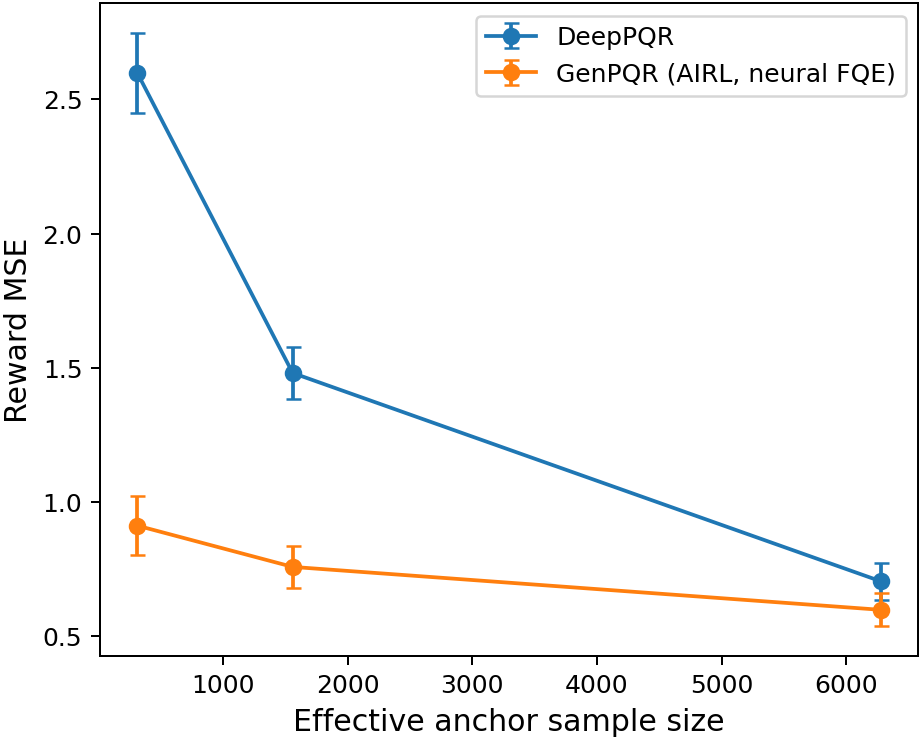
\includegraphics[width=\linewidth]{exp1_matched_curve.png}
\end{minipage}
\caption{Matched DeepPQR vs.\ GenPQR comparison. Both methods use the same AIRL policy estimate and neural FQE. Table entries are mean $\pm$ 95\% confidence interval over 100 seeds. Anchor count is the effective number of anchor-action transitions used by DeepPQR's anchor-$Q$ step.}
\label{fig:exp1_combo}
\end{figure*}



\paragraph{Method Comparison}
Our second experiment studies estimator choice at \(1000\) training trajectories with a well-supported anchor action. We compare AIRL versus behavior cloning for policy estimation, neural versus boosted fitted-\(Q\) evaluation, and include DeepPQR and standard reward-recovery baselines. Figure~\ref{fig:exp2_combo} shows that the modular GenPQR formulation remains effective across estimator choices, while runtime varies substantially across implementations.


\begin{figure}[htb]
\centering
\scriptsize
\setlength{\tabcolsep}{3pt}
\begin{tabular}{lcccc}
\toprule
Method & MSE $\downarrow$ & Corr. $\uparrow$ & NLL $\downarrow$ & Time $\downarrow$ \\
\midrule
GenPQR (BC, NN) & \textbf{0.37 $\pm$ 0.06} & \textbf{0.81 $\pm$ 0.01} & \textbf{1.546 $\pm$ 0.004} & 4.74 $\pm$ 0.06 \\
GenPQR (AIRL, NN) & 0.63 $\pm$ 0.06 & 0.72 $\pm$ 0.03 & 1.608 $\pm$ 0.006 & 26.43 $\pm$ 0.34 \\
GenPQR (BC, GBT) & 1.07 $\pm$ 0.19 & 0.49 $\pm$ 0.03 & \textbf{1.546 $\pm$ 0.004} & \textbf{2.25 $\pm$ 0.03} \\
GenPQR (AIRL, GBT) & 1.07 $\pm$ 0.19 & 0.41 $\pm$ 0.05 & 1.608 $\pm$ 0.006 & 23.97 $\pm$ 0.32 \\
\midrule
DeepPQR & 0.79 $\pm$ 0.07 & 0.69 $\pm$ 0.02 & 1.608 $\pm$ 0.006 & 38.24 $\pm$ 0.42 \\
MaxEnt-IRL & 1.17 $\pm$ 0.18 & 0.35 $\pm$ 0.03 & 1.624 $\pm$ 0.005 & 8.57 $\pm$ 0.11 \\
AIRL state reward & 2.17 $\pm$ 0.21 & -0.01 $\pm$ 0.03 & 1.608 $\pm$ 0.006 & 23.83 $\pm$ 0.32 \\
Log-policy pseudo & 3.40 $\pm$ 0.18 & 0.37 $\pm$ 0.05 & 1.608 $\pm$ 0.006 & 23.83 $\pm$ 0.32 \\
\bottomrule
\end{tabular}
\caption{Higher-sample method comparison. Entries are mean $\pm$ 95\% confidence interval over 100 seeds. NN = neural FQE; GBT = boosted FQE.}
\label{fig:exp2_combo}
\end{figure}


\textbf{Discussion.} Across the two studies, the matched comparison isolates the statistical cost of anchor-subset identification, while the higher-sample comparison shows that GenPQR remains effective across practical estimator choices.



  

 
\bibliographystyle{plainnat}
\bibliography{references}


\appendix
 


 


\section{Simulation Details}
\label{app:simulation-details}

This appendix summarizes the simulation design and implementation choices used
in Section~\ref{sec:experiments}. The full experiment scripts, configuration
choices, and plotting code are included in the accompanying repository.

\paragraph{Environment.}
We adapt the synthetic environment of \citet{geng2020deep}. States are
continuous with dimension \(p=5\), the action set has \(|\mathcal A|=5\)
actions, and the discount factor is \(\gamma=0.9\). We use an infinite-horizon
stationary data-generating process and generate finite trajectories of length
\(10\) for offline training and evaluation. The normalization is the anchor
constraint \(r(s,a^\dagger)=0\), implemented as anchor-action normalization
with \(a^\dagger=0\) and \(g(s)=0\). Train and test sets within each seed are
generated from the same underlying MDP parameters, with independent rollouts.

\paragraph{Behavior policy and transitions.}
The logged policy is generated from a soft \(Q\)-planner with \(\alpha=1\), so
that the DeepPQR log-policy identity is correctly matched. The planner induces
a heterogeneous but non-degenerate behavior policy, and we vary anchor support
by shifting the anchor-action logit. Transitions are deterministic conditional
on state and action up to boundary handling: actions induce action-specific
state shifts, and trajectories that leave the bounded state region are reset
uniformly within that region. We clip estimated action probabilities to
\([0.01,0.99]\) and renormalize before using them in either GenPQR or DeepPQR.

\paragraph{Experiment 1.}
The matched DeepPQR-vs.-GenPQR comparison uses shared AIRL policy estimation
and neural downstream approximation. We consider three settings:
\texttt{(200, -1.0)}, \texttt{(1000, -1.0)}, and \texttt{(2500, 0.0)}, where
the first entry is the number of training trajectories and the second is the
anchor-logit shift. These correspond to low-sample rare-anchor, mid-sample
rare-anchor, and high-sample common-anchor regimes. Each setting uses \(300\)
test trajectories and \(100\) random seeds.

\paragraph{Experiment 2.}
The higher-sample comparison fixes \(1000\) training trajectories, \(300\) test
trajectories, and anchor-logit shift \(0.0\), again over \(100\) seeds. We
compare DeepPQR, GenPQR with two policy estimators and two \(Q\)-estimators,
and several reward-recovery baselines that are standard in the IRL literature.

\paragraph{Policy estimators.}
AIRL uses a standard action-independent reward network and potential network,
both implemented as two-layer ReLU MLPs with hidden widths \((64,64)\), Adam
step size \(10^{-3}\), \(60\) behavior-cloning warm-start epochs, and \(80\)
adversarial updates in the paper experiments. Behavior cloning uses the same
\((64,64)\) MLP architecture and \(40\) epochs in Experiment~2. MaxEnt-IRL is
implemented as a neural softmax-\(Q\) model with hidden widths \((128,128)\)
and \(150\) gradient steps. These architectures were chosen to be standard for
low-dimensional synthetic control problems and to remain stable across seeds;
larger networks did not materially improve performance in pilot runs.

\paragraph{\(Q\)-evaluation.}
Neural FQE uses a dueling-style MLP \(Q(s,a)=V(s)+A(s,a)-\bar A(s)\) with
hidden widths \((128,128)\), Adam step size \(5\times 10^{-3}\), \(8\) Bellman
iterations, and \(4\) epochs of regression per iteration. Boosted FQE uses
LightGBM directly, with \(4\) outer Bellman iterations and \(30\) boosting
rounds per iteration, learning rate \(0.05\), \(32\) leaves, and minimum leaf
size \(20\). We selected these settings to balance Bellman-fit accuracy,
runtime, and seed-to-seed stability; the boosted configuration follows the
repository's adapted FQE implementation and avoids long inner re-fitting loops.

\paragraph{DeepPQR and baselines.}
DeepPQR uses the same shared AIRL policy estimate as GenPQR in the matched
comparison. It then estimates the anchor \(Q\)-function on the anchor-action
subset, reconstructs the full \(Q\)-function from log-policy ratios, and fits
the final reward-regression network. The AIRL state-reward baseline uses the
AIRL reward head directly; the log-policy pseudo-reward baseline uses
\(\log \hat\pi(a\mid s)-g(s)\); MaxEnt-IRL uses its learned \(Q\)-surrogate as
reward; and the linear reward baseline fits a strictly linear state-action
reward model with action-specific coefficients and ridge regularization.

\paragraph{Reporting.}
For each method we report reward mean squared error, reward correlation with
the ground-truth normalized reward, held-out policy negative log-likelihood
when applicable, and wall-clock runtime. Confidence intervals are normal
approximation intervals based on the \(100\) seed-level estimates.

 




\section{Additional Experimental Results}

\label{app:additional-experiments}


 
 
 

This appendix reports a supplemental study that
studies the many-action regime, where the number of actions grows while the
overall sample size is held fixed, so the effective anchor sample size for
DeepPQR decreases mechanically.

\paragraph{Method comparison.} Figure~\ref{fig:exp2_methods} corresponds to the second experiment in the main text.

\begin{figure}[htb]
\centering
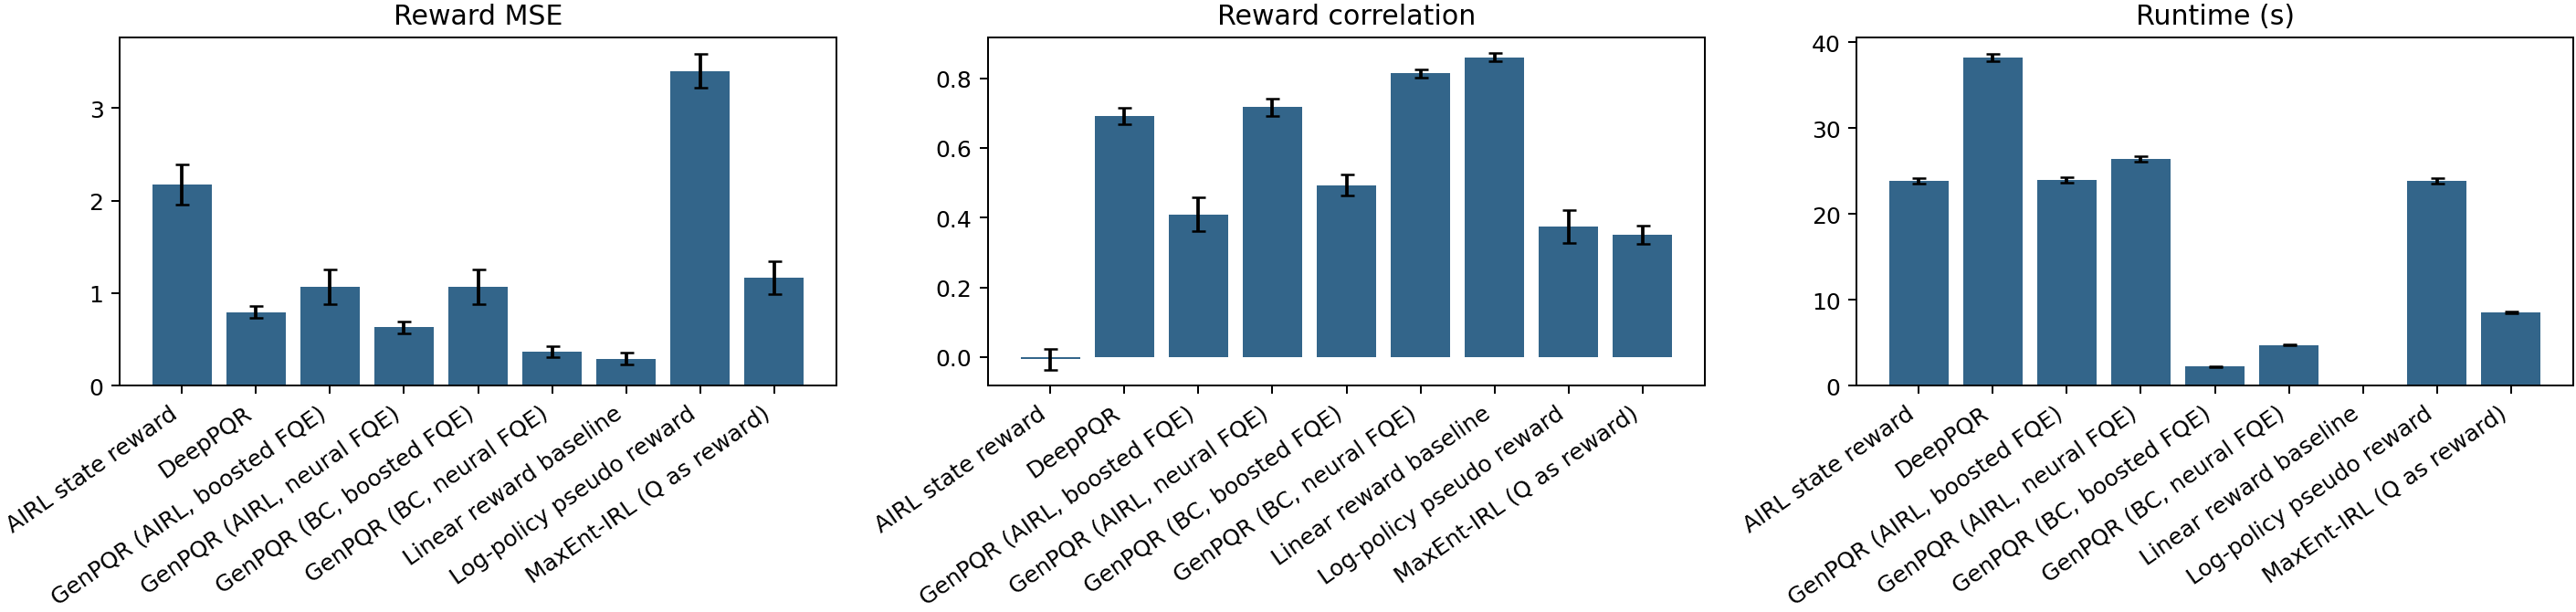
\includegraphics[width=0.95\linewidth]{exp2_method_comparison.png}
\caption{Higher-sample method comparison. Neural GenPQR variants outperform non-identifying baselines, and behavior cloning with neural FQE provides the best accuracy-runtime tradeoff in this setting. Error bars denote 95\% confidence intervals over 100 seeds.}
\label{fig:exp2_methods}
\end{figure}



 

\paragraph{Many-action regime.}
Figure~\ref{fig:app-many-action} fixes the overall sample size at the
high-sample matched setting and increases the number of actions. As
\(|\mathcal A|\) grows, the effective anchor sample size falls from roughly
\(6400\) anchor-action transitions at \(|\mathcal A|=5\) to roughly \(800\) at
\(|\mathcal A|=40\). In this regime, DeepPQR degrades sharply, whereas GenPQR
remains substantially more stable because its \(Q\)-evaluation step continues
to use the full sample. We show both AIRL- and BC-based versions of each
method. Because this fixed-sample action-scaling study was run as a quick pilot
to validate the trend, the figure should be interpreted as directional.

\begin{figure*}[htb]
\centering
\begin{minipage}[c]{0.48\textwidth}
\centering
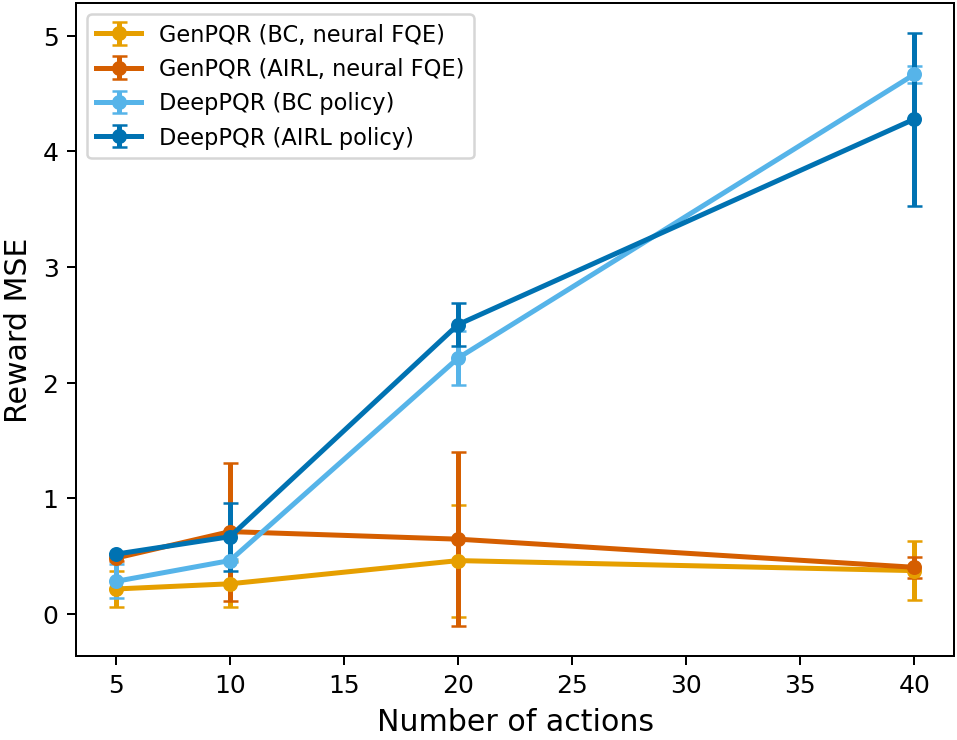
\includegraphics[width=\linewidth]{many_action_reward_mse.png}
\end{minipage}
\hfill
\begin{minipage}[c]{0.48\textwidth}
\centering
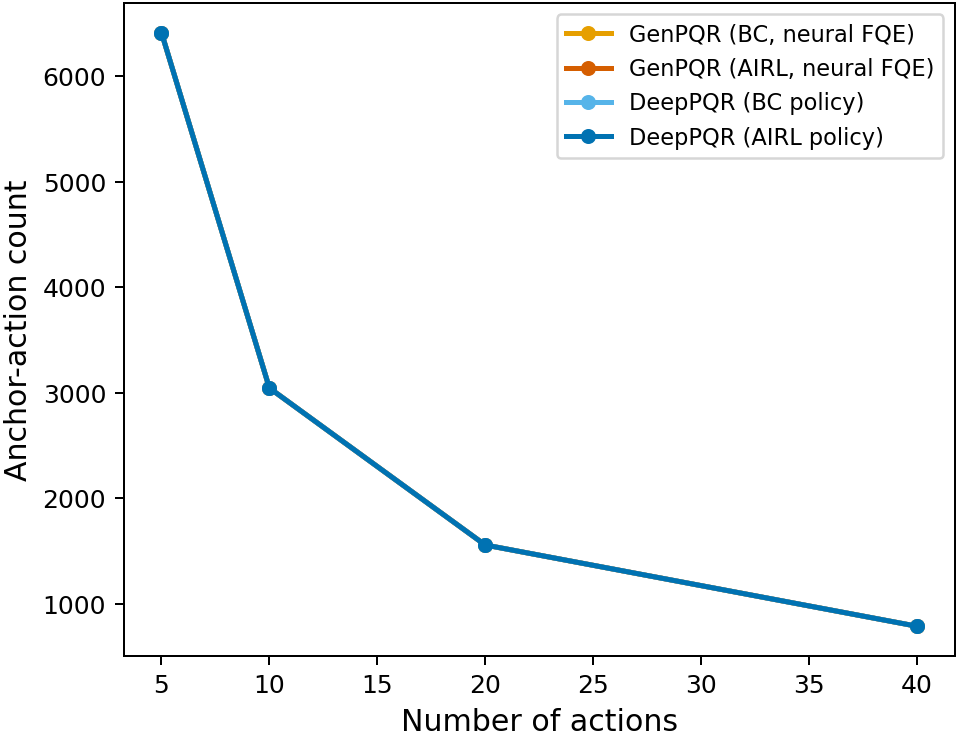
\includegraphics[width=\linewidth]{many_action_anchor_count.png}
\end{minipage}
\caption{Fixed-sample many-action study. Left: reward MSE as the number of actions increases. Right: realized anchor-action count over the same sweep. The total sample size is held fixed, so DeepPQR's effective sample size shrinks with \(|\mathcal A|\) while GenPQR continues to use the full sample in its \(Q\)-evaluation step.}
\label{fig:app-many-action}
\end{figure*}




\section{Identification and Representation}
\label{app:identification}

\subsection{Proof of Lemma~\ref{lem:trivial}}

\begin{proof}
Let \(u^\star(s,a):=\log \pi(a\mid s)\). Since
\[
\sum_{a'}\exp\{u^\star(s,a')\}
=
\sum_{a'} \pi(a'\mid s)
=
1,
\]
we have \(\Xi(u^\star)(s)=0\) for every \(s\). Hence
\[
P\Xi(u^\star)(s,a)=0,
\]
so \((u^\star,0)\) is feasible for \eqref{eq:relaxed-irl}.

To prove optimality, define \(q(s,a):=r(s,a)+\gamma v(s,a)\). For any feasible
\((r,v)\), the objective in \eqref{eq:relaxed-irl} can be written as
\[
\E_{(s,a)\sim \nu_\pi}\!\big[q(s,a)-\Xi q(s)\big].
\]
For each state \(s\), the quantity \(q(s,a)-\Xi q(s)\) is the log-probability
of action \(a\) under the softmax policy induced by \(q\),
\[
\pi_q(a\mid s)
:=
\exp\{q(s,a)-\Xi q(s)\}.
\]
Therefore
\begin{align*}
\E_{(s,a)\sim \nu_\pi}\!\big[q(s,a)-\Xi q(s)\big]
&=
\E_{s\sim \rho}\!\left[
\sum_a \pi(a\mid s)\log \pi_q(a\mid s)
\right] \\
&=
-\E_{s\sim \rho}\!\Bigl[
\KL\!\bigl(\pi(\cdot\mid s)\,\|\,\pi_q(\cdot\mid s)\bigr)
\Bigr]
+ \E_{s\sim \rho}\!\bigl[H(\pi(\cdot\mid s))\bigr].
\end{align*}
This is maximized when \(\pi_q(\cdot\mid s)=\pi(\cdot\mid s)\) for every
\(s\), which is attained by \(q=u^\star\), i.e., by \((r,v)=(u^\star,0)\).
\end{proof}

\subsection{Proof of Lemma~\ref{lem:shaping}}

\begin{proof}
Let \(q:=r+\gamma v\), and define
\[
\tilde r=r+c-\gamma Pc,
\qquad
\tilde v=v+Pc.
\]
Then
\[
\tilde r+\gamma \tilde v
=
r+\gamma v + c
=
q+c,
\]
where \(c\) is understood as a state-only function added to every action at
the same state. Consequently,
\[
\Xi(\tilde r+\gamma\tilde v)(s)
=
\Xi(q+c)(s)
=
c(s)+\Xi q(s).
\]
Applying \(P\) to both sides gives
\[
P\Xi(\tilde r+\gamma\tilde v)
=
Pc + P\Xi q
=
Pc + v
=
\tilde v,
\]
so \((\tilde r,\tilde v)\) is feasible for \eqref{eq:relaxed-irl}.

The objective value is unchanged because
\[
\tilde r(s,a)+\gamma \tilde v(s,a)-\Xi(\tilde r+\gamma\tilde v)(s)
=
q(s,a)+c(s)-\bigl(\Xi q(s)+c(s)\bigr)
=
q(s,a)-\Xi q(s).
\]
Thus \((\tilde r,\tilde v)\) attains the same objective value as \((r,v)\).
The induced log-policy,
\[
\tilde r+\gamma \tilde v-\Xi(\tilde r+\gamma\tilde v)
=
q-\Xi q,
\]
is therefore also unchanged.
\end{proof}

\subsection{Proof of Theorem~\ref{thm:unique}}

\begin{proof}
Let \(Q^\mu_{u^\star-g}\) denote the unique bounded fixed point of
\[
Q = u^\star-g+\gamma P\mu Q.
\]
Define
\[
r^\star
:=
Q^\mu_{u^\star-g}-\mu Q^\mu_{u^\star-g}+g,
\qquad
v^\star
:=
\frac{1}{\gamma}\bigl(u^\star-g-Q^\mu_{u^\star-g}\bigr).
\]

We first verify feasibility for \eqref{eq:main-irl}. The normalization is
immediate:
\[
\mu r^\star
=
\mu Q^\mu_{u^\star-g}-\mu Q^\mu_{u^\star-g}+g
=
g.
\]
Next, the Bellman equation for \(Q^\mu_{u^\star-g}\) implies
\[
v^\star
=
\frac{1}{\gamma}\bigl(u^\star-g-Q^\mu_{u^\star-g}\bigr)
=
-P\mu Q^\mu_{u^\star-g}.
\]
Hence
\[
r^\star+\gamma v^\star
=
Q^\mu_{u^\star-g}-\mu Q^\mu_{u^\star-g}+g
+
u^\star-g-Q^\mu_{u^\star-g}
=
u^\star-\mu Q^\mu_{u^\star-g}.
\]
Since \(\mu Q^\mu_{u^\star-g}\) is state-only and \(\Xi(u^\star)=0\),
\[
\Xi(r^\star+\gamma v^\star)
=
\Xi\!\bigl(u^\star-\mu Q^\mu_{u^\star-g}\bigr)
=
-\mu Q^\mu_{u^\star-g}.
\]
Applying \(P\) gives
\[
P\Xi(r^\star+\gamma v^\star)
=
-P\mu Q^\mu_{u^\star-g}
=
v^\star.
\]
Thus \((r^\star,v^\star)\) is feasible.

To prove optimality, observe that
\[
r^\star+\gamma v^\star
=
u^\star+c^\star,
\qquad
c^\star(s):= -(\mu Q^\mu_{u^\star-g})(s).
\]
By the same log-likelihood argument as in Lemma~\ref{lem:trivial}, adding a
state-only shift \(c^\star\) does not change the induced policy, so
\((r^\star,v^\star)\) attains the same objective value as \((u^\star,0)\).
Hence it is optimal.

It remains to show uniqueness. Let \((r,v)\) be any optimal feasible pair for
\eqref{eq:main-irl}, and set \(q:=r+\gamma v\). Since \((r,v)\) is also
feasible for the relaxed problem and achieves the same maximal likelihood as
\((u^\star,0)\), the induced policy must equal \(\pi\). Therefore
\[
u^\star(s,a)
=
q(s,a)-\Xi q(s),
\]
which implies
\[
q(s,a)=u^\star(s,a)+c(s),
\qquad
c(s):=\Xi q(s).
\]
Feasibility then gives
\[
v
=
P\Xi q
=
Pc,
\qquad
r
=
q-\gamma v
=
u^\star+c-\gamma Pc.
\]
The normalization condition \(\mu r=g\) becomes
\[
g
=
\mu u^\star + c - \gamma P_\mu c,
\qquad
P_\mu c(s):=\int Pc(s,a)\,\mu(da\mid s).
\]
Equivalently,
\[
(I-\gamma P_\mu)c
=
g-\mu u^\star.
\]
Since \(P_\mu\) is a Markov operator with \(\|P_\mu\|_\infty\le 1\) and
\(\gamma<1\), the operator \(I-\gamma P_\mu\) is invertible on bounded
functions via the Neumann series. Thus \(c\) is unique, and so are \(v=Pc\)
and \(r=u^\star+c-\gamma Pc\).
\end{proof}

\subsection{An Equivalent Identification}

The next result rewrites the identification in terms of the continuation value
\(v^\star\). It is equivalent to Theorem~\ref{thm:unique}, but it enables direct
modeling of \(v^\star\), from which the reward \(r^\star\) is obtained
immediately.


\begin{theorem}[An equivalent identification with anchor function]
\label{thm:unique2}
\Cref{eq:main-irl} admits a unique optimal solution \((r^\star,v^\star)\), where
\[
r^\star
=
\ustar + \mu\!\left(g+\gamma v^\star-\ustar\right)-\gamma v^\star,
\]
and \(v^\star\) is the unique bounded solution to the fixed-point equation
\[
v^\star = P\mu\!\left(g+\gamma v^\star-\ustar\right).
\]
\end{theorem}

\begin{proof}
Let \(Q^\mu_{\ustar-g}\) denote the unique bounded solution to
\[
Q^\mu_{\ustar-g}
=
\ustar-g+\gamma P\mu Q^\mu_{\ustar-g}.
\]
By Theorem~\ref{thm:unique},
\[
r^\star
=
Q^\mu_{\ustar-g}-\mu Q^\mu_{\ustar-g}+g,
\qquad
v^\star
=
\frac{1}{\gamma}\bigl(\ustar-g-Q^\mu_{\ustar-g}\bigr).
\]
Equivalently,
\[
Q^\mu_{\ustar-g}=\ustar-g-\gamma v^\star.
\]
Substituting this identity into the Bellman equation for \(Q^\mu_{\ustar-g}\)
gives
\[
\ustar-g-\gamma v^\star
=
\ustar-g+\gamma P\mu(\ustar-g-\gamma v^\star),
\]
hence
\[
v^\star
=
-P\mu(\ustar-g-\gamma v^\star)
=
P\mu(g+\gamma v^\star-\ustar),
\]
which is the claimed fixed-point equation.

For the reward,
\begin{align*}
r^\star
&=
Q^\mu_{\ustar-g}-\mu Q^\mu_{\ustar-g}+g \\
&=
(\ustar-g-\gamma v^\star)-\mu(\ustar-g-\gamma v^\star)+g \\
&=
\ustar + \mu(g+\gamma v^\star-\ustar)-\gamma v^\star.
\end{align*}
Uniqueness follows directly from Theorem~\ref{thm:unique}.
\end{proof}


\subsection{Proof of Theorem~\ref{thm:identification}}

\begin{proof}
Let \((r,v)\) solve \eqref{eq:relaxed-irl}, and define
\[
q:=r+\gamma v,
\qquad
c(s):=\Xi q(s).
\]
Since \((r,v)\) is optimal for the relaxed problem, it induces the behavior
policy \(\pi\). Therefore
\[
u^\star(s,a)
=
q(s,a)-\Xi q(s)
=
q(s,a)-c(s),
\]
so
\[
q(s,a)=u^\star(s,a)+c(s).
\]
The Bellman feasibility condition then gives
\[
v=P\Xi q=Pc,
\qquad
r=q-\gamma v=u^\star+c-\gamma Pc.
\]

Fix any policy \(\pi_1\), and let \(Q^\pi_{u^\star}\) denote the unique bounded
solution to
\[
Q^\pi_{u^\star}
=
u^\star+\gamma \pi_1 P Q^\pi_{u^\star}.
\]
Because \(c\) is state-only,
\[
\pi_1 P c = Pc.
\]
Hence
\begin{align*}
r+\gamma \pi_1 P\bigl(Q^\pi_{u^\star}+c\bigr)
&=
u^\star+c-\gamma Pc+\gamma \pi_1 P Q^\pi_{u^\star}+\gamma \pi_1 P c \\
&=
u^\star+\gamma \pi_1 P Q^\pi_{u^\star}+c \\
&=
Q^\pi_{u^\star}+c.
\end{align*}
So \(Q^\pi_{u^\star}+c\) solves the Bellman equation for reward \(r\) under
policy \(\pi_1\). By uniqueness of bounded Bellman fixed points,
\[
Q_r^{\pi_1}=Q_{u^\star}^{\pi_1}+c,
\]
which is equivalent to
\[
Q_{u^\star}^{\pi_1}=Q_r^{\pi_1}-c.
\]

Now let \(c^\star\) denote the state shift corresponding to the normalized
solution \(r^\star\). By Theorem~\ref{thm:unique}, \(r^\star\) is also a shaped
version of \(u^\star\), so the same argument gives
\[
Q_{r^\star}^{\pi_i}=Q_{u^\star}^{\pi_i}+c^\star,
\qquad i\in\{1,2\}.
\]
Taking policy values and using that \(c\) and \(c^\star\) are state-only,
\[
V_r^{\pi_i}
=
V_{u^\star}^{\pi_i}+c,
\qquad
V_{r^\star}^{\pi_i}
=
V_{u^\star}^{\pi_i}+c^\star.
\]
Subtracting the identities for \(i=1\) and \(i=2\) proves
\[
V_{r^\star}^{\pi_1}(s)-V_{r^\star}^{\pi_2}(s)
=
V_r^{\pi_1}(s)-V_r^{\pi_2}(s).
\qedhere
\]
\end{proof}

\section{Reward Recovery and Finite-Sample Analysis}
\label{app:recovery}

\subsection{Proof of Theorem~\ref{thm:reward-recovery}}

\begin{proof}
For any measure \(d\) on \(\mathcal S\), let
\(
\|h\|_{2,d} := \{\E_{s\sim d}[h(s)^2]\}^{1/2}.
\)
Since
\(
r^\star(s,a)=Q^\mu_{u^\star-g}(s,a)-(\mu Q^\mu_{u^\star-g})(s)+g(s),
\)
we may write
\(
r^\star-\hat r=\widetilde\Delta_Q-\mu\widetilde\Delta_Q,
\)
where
\(
\widetilde\Delta_Q:=Q^\mu_{u^\star-g}-\hat Q.
\)
Therefore
\begin{equation}
\label{eq:reward-split}
\|r^\star-\hat r\|_{2,\mathrm{beh}}
\le
\|\widetilde\Delta_Q\|_{2,\mathrm{beh}}
+
\|\mu\widetilde\Delta_Q\|_{2,\mathrm{beh}}.
\end{equation}

For any measurable \(f:\mathcal S\times\mathcal A\to\mathbb R\), Jensen's inequality gives
\[
|\mu f(s)|^2
=
\Bigl|\sum_a \mu(a\mid s)f(s,a)\Bigr|^2
\le
\sum_a \mu(a\mid s)f(s,a)^2.
\]
Hence
\[
\|\mu f\|_{2,\mathrm{beh}}^2
\le
\int \sum_a \mu(a\mid s)f(s,a)^2\,d\rho(s)
=
\int \frac{\mu(a\mid s)}{\pi(a\mid s)}f(s,a)^2\,d\nu_\pi(s,a)
\le
C_{\mu/\pi}\|f\|_{2,\mathrm{beh}}^2,
\]
so
\(
\|\mu f\|_{2,\mathrm{beh}}
\le
\sqrt{C_{\mu/\pi}}\|f\|_{2,\mathrm{beh}}.
\)
Applying this to \eqref{eq:reward-split} yields
\begin{equation}
\label{eq:reward-to-Q}
\|r^\star-\hat r\|_{2,\mathrm{beh}}
\le
(1+\sqrt{C_{\mu/\pi}})\|\widetilde\Delta_Q\|_{2,\mathrm{beh}}.
\end{equation}

Now let
\(
\Delta Q:=Q^\mu_{u^\star-g}-Q^\mu_{\hat u-g}
\)
and
\(
\Delta u:=u^\star-\hat u.
\)
Then
\begin{equation}
\label{eq:Q-triangle}
\|\widetilde\Delta_Q\|_{2,\mathrm{beh}}
\le
\|Q^\mu_{\hat u-g}-\hat Q\|_{2,\mathrm{beh}}
+
\|\Delta Q\|_{2,\mathrm{beh}}.
\end{equation}
Subtracting the Bellman equations gives
\(
\Delta Q=\Delta u+\gamma P\mu\,\Delta Q,
\)
hence
\(
\|\Delta Q\|_{2,\mathrm{beh}}
\le
\|\Delta u\|_{2,\mathrm{beh}}+\gamma\|P\mu\,\Delta Q\|_{2,\mathrm{beh}}.
\)

Using Jensen again, \((P\mu \Delta Q)^2 \le P\mu((\Delta Q)^2)\), so
\begin{align}
\|P\mu\,\Delta Q\|_{2,\mathrm{beh}}^2
&\le
\int P\mu\bigl((\Delta Q)^2\bigr)\,d\nu_\pi
=
\int (\Delta Q)^2\,d(\nu_\pi P\mu) \notag\\
&=
\int \sum_a (\Delta Q(s,a))^2\mu(a\mid s)\,d(\nu_\pi P)(s) \notag\\
&\le
C_{\nu_\pi P/d_\mu}
\int \sum_a (\Delta Q(s,a))^2\mu(a\mid s)\,dd_\mu(s).
\label{eq:pmu-mixed}
\end{align}
Define the mixed norm
\[
\|f\|_{2,d_\mu,\mu}
:=
\left\{
\int \sum_a f(s,a)^2\mu(a\mid s)\,d_\mu(s)
\right\}^{1/2}.
\]
Then \eqref{eq:pmu-mixed} implies
\begin{equation}
\label{eq:DeltaQ-beh}
\|\Delta Q\|_{2,\mathrm{beh}}
\le
\|\Delta u\|_{2,\mathrm{beh}}
+
\gamma\sqrt{C_{\nu_\pi P/d_\mu}}\,
\|\Delta Q\|_{2,d_\mu,\mu}.
\end{equation}

It remains to control \(\|\Delta Q\|_{2,d_\mu,\mu}\). Taking \(\|\cdot\|_{2,d_\mu,\mu}\) norms in
\(
\Delta Q=\Delta u+\gamma P\mu\,\Delta Q
\)
gives
\(
\|\Delta Q\|_{2,d_\mu,\mu}
\le
\|\Delta u\|_{2,d_\mu,\mu}
+
\gamma\|P\mu\,\Delta Q\|_{2,d_\mu,\mu}.
\)
Because \(d_\mu\) is stationary for \(P_\mu\), Jensen's inequality yields
\(
\|P\mu f\|_{2,d_\mu,\mu}\le \|f\|_{2,d_\mu,\mu}
\)
for all \(f\). Therefore
\[
(1-\gamma)\|\Delta Q\|_{2,d_\mu,\mu}
\le
\|\Delta u\|_{2,d_\mu,\mu}.
\]

Finally,
\begin{align*}
\|\Delta u\|_{2,d_\mu,\mu}^2
&=
\int (\Delta u(s,a))^2\,d_\mu(s)\mu(da\mid s) \\
&=
\int (\Delta u(s,a))^2
\frac{dd_\mu}{d\rho}(s)\frac{\mu(a\mid s)}{\pi(a\mid s)}
\,d\nu_\pi(s,a) \\
&\le
C_{d_\mu/\rho}C_{\mu/\pi}\|\Delta u\|_{2,\mathrm{beh}}^2.
\end{align*}
Thus
\begin{equation}
\label{eq:DeltaQ-lambda}
\|\Delta Q\|_{2,d_\mu,\mu}
\le
\frac{\sqrt{C_{d_\mu/\rho}C_{\mu/\pi}}}{1-\gamma}
\|u^\star-\hat u\|_{2,\mathrm{beh}}.
\end{equation}

Combining \eqref{eq:Q-triangle}, \eqref{eq:DeltaQ-beh}, and \eqref{eq:DeltaQ-lambda}, we obtain
\[
\|\widetilde\Delta_Q\|_{2,\mathrm{beh}}
\le
\|Q^\mu_{\hat u-g}-\hat Q\|_{2,\mathrm{beh}}
+
\left(
1+\frac{\gamma\sqrt{C_{\nu_\pi P/d_\mu}\,C_{d_\mu/\rho}C_{\mu/\pi}}}{1-\gamma}
\right)
\|u^\star-\hat u\|_{2,\mathrm{beh}}.
\]
Substituting this into \eqref{eq:reward-to-Q} proves the claim.
\end{proof}


\subsection{Technical Lemmas}
\label{appendix:lemmas}

\begin{lemma}
\label{lemma::KLell2}
Under Assumption~\ref{assump:policy-gen}, suppose additionally that there
exists \(\underline p>0\) such that, with probability at least \(1-\delta\),
\[
\pi(a\mid s)\ge \underline p
\quad\text{and}\quad
\hat\pi(a\mid s)\ge \underline p
\qquad\text{for all }(s,a).
\]
Then, for \(C_p:=\sqrt{2}\,\underline p^{-2}\), with probability at least
\(1-\delta\),
\[
\|\hat u-u^\star\|_{2, \mathrm{beh}}
\le
C_p\,\rho_{\pi}(n,\delta).
\]
\end{lemma}

\begin{proof}
Let \(u^\star=\log \pi\), \(\hat u=\log \hat\pi\), and define the likelihood
ratio
\[
\vartheta(a\mid s):=\frac{\hat\pi(a\mid s)}{\pi(a\mid s)}.
\]
Since \(\pi(a\mid s)\ge \underline p\) and \(\hat\pi(a\mid s)\ge \underline p\),
we have
\[
\vartheta(a\mid s)\in [\underline p, \underline p^{-1}]
\]
for all \((s,a)\).

Define \(\phi(t):=-\log t-(1-t)\). Since \(\phi''(t)=t^{-2}\), the function
\(\phi\) is \(\underline p^2\)-strongly convex on
\([\underline p,\underline p^{-1}]\). Also,
\(\E_{\pi(\cdot\mid s)}[\vartheta]=1\), so for each \(s\),
\begin{align*}
\mathrm{KL}\!\big(\pi(\cdot\mid s)\,\|\,\hat\pi(\cdot\mid s)\big)
&=
\E_{\pi(\cdot\mid s)}[-\log \vartheta]
=
\E_{\pi(\cdot\mid s)}[\phi(\vartheta)] \\
&\ge
\frac{\underline p^2}{2}\,
\E_{\pi(\cdot\mid s)}[(\vartheta-1)^2].
\end{align*}
Moreover, by the mean value theorem, for \(t\in[\underline p,\underline p^{-1}]\),
\[
|\log t|
\le
\underline p^{-1} |t-1|.
\]
Applying this with \(t=\vartheta\) gives
\begin{align*}
\E_{\pi(\cdot\mid s)}\big[(\hat u-u^\star)^2\big]
&=
\E_{\pi(\cdot\mid s)}\big[(\log \vartheta)^2\big] \\
&\le
\underline p^{-2}\,\E_{\pi(\cdot\mid s)}\big[(\vartheta-1)^2\big] \\
&\le
2\underline p^{-4}\,
\mathrm{KL}\!\big(\pi(\cdot\mid s)\,\|\,\hat\pi(\cdot\mid s)\big).
\end{align*}
Averaging over \(s\) and invoking Assumption~\ref{assump:policy-gen} yields
\[
\|\hat u-u^\star\|_{2,\mathrm{beh}}
\le
\sqrt{2}\,\underline p^{-2}
\left\{
\E_s\!\left[
\mathrm{KL}\!\big(\pi(\cdot\mid s)\,\|\,\hat\pi(\cdot\mid s)\big)
\right]
\right\}^{1/2}
\le
C\,\rho_{\pi}(n,\delta),
\]
where \(C:=\sqrt{2}\,\underline p^{-2}\).
\end{proof}

\begin{lemma}[Per-iteration error bound]
\label{lemma::periter}
Under Assumptions~\ref{assump:policy-gen}--\ref{assump:q-gen}, there exists a
constant \(C \in (0,\infty)\) such that, with probability at least \(1-\delta\),
\[
\|\mathcal T_{\hat u}^\mu(\hat Q^{(k-1)})-\hat Q^{(k)}\|_{2,\mathrm{beh}}
\le
\sqrt{2}\underline p^{-2}\,\rho_\pi(n,\delta)+\rho_{Q}(n,\delta)+\varepsilon_{\mathcal F}.
\]
\end{lemma}

\begin{proof}
Use \(\|\cdot\|\) to denote \(\|\cdot\|_{2,\mathrm{beh}}\). Let
\[
R_k
:=
\|\mathcal T_{\hat u}^\mu(\hat Q^{(k-1)})-\hat Q^{(k)}\|,
\qquad
R_k^\star
:=
\inf_{f\in\mathcal F}
\|\mathcal T_{\hat u}^\mu(\hat Q^{(k-1)})-f\|.
\]
By definition of the regret and Assumption~\ref{assump:q-gen}, with probability
at least \(1-\delta/2\),
\[
R_k^2-(R_k^\star)^2
=
\mathrm{reg}(\hat Q^{(k)}\mid \hat u,\hat Q^{(k-1)})
\le
\rho_{Q}(n,\delta/2)^2.
\]
Since
\[
R_k^2-(R_k^\star)^2=(R_k-R_k^\star)(R_k+R_k^\star)\ge (R_k-R_k^\star)^2,
\]
it follows that
\[
R_k
\le
R_k^\star+\rho_{Q}(n,\delta/2).
\]

Moreover, for any \(f\in\mathcal F\),
\begin{align*}
\|\mathcal T_{\hat u}^\mu(\hat Q^{(k-1)})-f\|
&\le
\|\mathcal T_{\hat u}^\mu(\hat Q^{(k-1)})
-\mathcal T_{u^\star}^\mu(\hat Q^{(k-1)})\| \\
&\quad+
\|\mathcal T_{u^\star}^\mu(\hat Q^{(k-1)})-f\| \\
&=
\|\hat u-u^\star\|
+
\|\mathcal T_{u^\star}^\mu(\hat Q^{(k-1)})-f\|.
\end{align*}
Taking the infimum over \(f\in\mathcal F\) yields
\[
R_k^\star
\le
\|\hat u-u^\star\|
+
\inf_{f\in\mathcal F}
\|\mathcal T_{u^\star}^\mu(\hat Q^{(k-1)})-f\|.
\]
Since \(\nu_\pi\) is a probability measure,
\[
\|h\|_{2,\mathrm{beh}}\le \|h\|_\infty
\qquad\text{for all }h,
\]
so by the definition of \(\varepsilon_{\mathcal F}\),
\[
\inf_{f\in\mathcal F}
\|\mathcal T_{u^\star}^\mu(\hat Q^{(k-1)})-f\|
\le
\inf_{f\in\mathcal F}
\|\mathcal T_{u^\star}^\mu(\hat Q^{(k-1)})-f\|_\infty
\le
\varepsilon_{\mathcal F}.
\]
Therefore, with probability at least \(1-\delta/2\),
\[
\|\mathcal T_{\hat u}^\mu(\hat Q^{(k-1)})-\hat Q^{(k)}\|
\le
\rho_{Q}(n,\delta/2)+\|\hat u-u^\star\|+\varepsilon_{\mathcal F}.
\]

Finally, Lemma~\ref{lemma::KLell2} implies that, with probability at least
\(1-\delta/2\),
\[
\|\hat u-u^\star\|_{2,\mathrm{beh}}
\le
\sqrt{2}\underline p^{-2}\,\rho_\pi(n,\delta/2)
\]
for a constant \(C \in (0,\infty)\) depending only on the bounded-logit
constant in Assumption~\ref{assump:policy-gen}. A union bound gives the
claimed inequality.
\end{proof}

\begin{assumption}[Concentrability of propagated state-action distributions]
\label{assump:fqe-conc}
Assume that
\[
C_{\mathrm{conc}}
:=
\sup_{m\ge 0}
\left\|
\frac{d\bigl(\nu_\pi (P\mu)^m\bigr)}{d\nu_\pi}
\right\|_\infty
< \infty.
\]
\end{assumption}



\begin{lemma}[Coverage implies propagated concentrability]
\label{lem:coverage-implies-conc}
Let \(\nu_\pi:=\rho\otimes \pi\) and \(\nu_\mu:=d_\mu\otimes \mu\), where
\(d_\mu\) is a stationary distribution of \(P_\mu\). Suppose that
\[
C_{\mu/\pi}
:=
\left\|
\frac{\mu(a\mid s)}{\pi(a\mid s)}
\right\|_\infty
<\infty,
\qquad
C_{d_\mu/\rho}
:=
\left\|
\frac{d d_\mu(s)}{d\rho(s)}
\right\|_\infty
<\infty,
\]
and
\[
C_{\nu_\pi P/d_\mu}
:=
\left\|
\frac{d(\nu_\pi P)(s)}{d d_\mu(s)}
\right\|_\infty
<\infty.
\]
Then
\[
\sup_{m\ge 0}
\left\|
\frac{d\bigl(\nu_\pi (P\mu)^m\bigr)}{d\nu_\pi}
\right\|_\infty
\le
\max\Bigl\{
1,\,
C_{\nu_\pi P/d_\mu}\,C_{d_\mu/\rho}\,C_{\mu/\pi}
\Bigr\}.
\]
In particular, Assumption~\ref{cond::coverage} implies
Assumption~\ref{assump:fqe-conc}.
\end{lemma}

\begin{proof}
For \(m=0\),
\[
\left\|
\frac{d\bigl(\nu_\pi (P\mu)^0\bigr)}{d\nu_\pi}
\right\|_\infty
=
\left\|
\frac{d\nu_\pi}{d\nu_\pi}
\right\|_\infty
=
1.
\]

Now fix \(m\ge 1\). Write
\[
\eta_m:= (\nu_\pi P)(P_\mu)^{m-1},
\]
so that
\[
\nu_\pi (P\mu)^m = \eta_m \otimes \mu.
\]
Since \(\nu_\pi=\rho\otimes\pi\), we have
\[
\frac{d\bigl(\nu_\pi (P\mu)^m\bigr)}{d\nu_\pi}(s,a)
=
\frac{d\eta_m}{d\rho}(s)\,
\frac{\mu(a\mid s)}{\pi(a\mid s)}.
\]
Using \(d_\mu\ll \rho\), this becomes
\[
\frac{d\bigl(\nu_\pi (P\mu)^m\bigr)}{d\nu_\pi}(s,a)
=
\frac{d\eta_m}{d d_\mu}(s)\,
\frac{d d_\mu}{d\rho}(s)\,
\frac{\mu(a\mid s)}{\pi(a\mid s)}.
\]
Hence
\[
\left\|
\frac{d\bigl(\nu_\pi (P\mu)^m\bigr)}{d\nu_\pi}
\right\|_\infty
\le
\left\|
\frac{d\eta_m}{d d_\mu}
\right\|_\infty
\left\|
\frac{d d_\mu}{d\rho}
\right\|_\infty
\left\|
\frac{\mu}{\pi}
\right\|_\infty.
\]

It remains to bound the first factor. Let
\[
h_0:=\frac{d(\nu_\pi P)}{d d_\mu}.
\]
Because \(d_\mu\) is stationary for \(P_\mu\), for every \(k\ge 0\),
\[
\frac{d\bigl((\nu_\pi P)(P_\mu)^k\bigr)}{d d_\mu}
=
P_\mu^k h_0,
\]
where \(P_\mu\) acts on bounded measurable functions by
\[
(P_\mu f)(s):=\int f(s')\,P_\mu(ds'\mid s).
\]
Therefore,
\[
\left\|
\frac{d\eta_m}{d d_\mu}
\right\|_\infty
=
\|P_\mu^{m-1} h_0\|_\infty
\le
\|h_0\|_\infty
=
\left\|
\frac{d(\nu_\pi P)}{d d_\mu}
\right\|_\infty
=
C_{\nu_\pi P/d_\mu},
\]
since a Markov operator is \(L^\infty\)-nonexpansive.

Thus, for all \(m\ge 1\),
\[
\left\|
\frac{d\bigl(\nu_\pi (P\mu)^m\bigr)}{d\nu_\pi}
\right\|_\infty
\le
C_{\nu_\pi P/d_\mu}\,
C_{d_\mu/\rho}\,
C_{\mu/\pi}.
\]
Combining this with the case \(m=0\) gives
\[
\sup_{m\ge 0}
\left\|
\frac{d\bigl(\nu_\pi (P\mu)^m\bigr)}{d\nu_\pi}
\right\|_\infty
\le
\max\Bigl\{
1,\,
C_{\nu_\pi P/d_\mu}\,C_{d_\mu/\rho}\,C_{\mu/\pi}
\Bigr\}.
\]
\end{proof}


\subsection{GenPQR + FQE Bound}

\paragraph{Boundedness condition for the FQE recursion.}
In addition to Assumptions~\ref{assump:policy-gen}--\ref{assump:q-gen},
assume that the regression class is uniformly bounded:
\[
\sup_{f\in\mathcal F}\|f\|_\infty \le B_{\mathcal F}<\infty.
\]
Assumption~\ref{assump:policy-gen} already gives
\(\|\hat u\|_\infty \vee \|u^\star\|_\infty \le B < \infty\), and \(g\) is bounded by
construction. Hence the Bellman targets \(\mathcal T^\mu_{\hat u}f\) are
uniformly bounded whenever \(f\in\mathcal F\) is. This is the standard
boundedness condition used in sup-norm FQE analyses.

 



\begin{lemma}[FQE error bound]
\label{lem:fqe-bound}
Let \(\mathcal T^\mu_u f := u-g+\gamma P\mu f\), and let
\(Q^\mu_{\hat u-g}\) denote the unique fixed point of
\(\mathcal T^\mu_{\hat u}\). Suppose \(\hat Q^{(k)}\) is produced by
Algorithm~\ref{alg:simple-irl}. Under
Assumptions~\ref{assump:policy-gen}--\ref{assump:q-gen},
Assumption~\ref{assump:fqe-conc}, and the boundedness condition above, then  with probability at least
\(1-\delta\),
\begin{align*}
\|Q^\mu_{\hat u-g}-\hat Q^{(K)}\|_{2,\mathrm{beh}}
&\le
\sqrt{C_{\mathrm{conc}}}\,\gamma^K
\|Q^\mu_{\hat u-g}-\hat Q^{(0)}\|_{\infty}\\
&\qquad+
\frac{\sqrt{C_{\mathrm{conc}}}}{1-\gamma}
\Bigl(
\varepsilon_{\mathcal F}
+\rho_Q(n,\delta/(2K))
+ \sqrt{2}\underline p^{-2}\,\rho_\pi(n,\delta/2)
\Bigr).
\end{align*}
\end{lemma}

\begin{proof}
Write \(Q_{\hat u}:=Q^\mu_{\hat u-g}\), and define
\[
\xi_k
:=
\mathcal T^\mu_{\hat u}\hat Q^{(k-1)}-\hat Q^{(k)}.
\]
Since \(Q_{\hat u}\) is the fixed point of \(\mathcal T^\mu_{\hat u}\),
\[
Q_{\hat u}-\hat Q^{(k)}
=
\mathcal T^\mu_{\hat u}(Q_{\hat u})
-\mathcal T^\mu_{\hat u}(\hat Q^{(k-1)})
+\xi_k
=
\gamma P\mu\bigl(Q_{\hat u}-\hat Q^{(k-1)}\bigr)+\xi_k.
\]
Iterating this recursion gives
\[
Q_{\hat u}-\hat Q^{(K)}
=
\gamma^K (P\mu)^K\bigl(Q_{\hat u}-\hat Q^{(0)}\bigr)
+
\sum_{j=1}^K \gamma^{K-j}(P\mu)^{K-j}\xi_j.
\]
Therefore,
\begin{align*}
\|Q_{\hat u}-\hat Q^{(K)}\|_{2,\mathrm{beh}}
\le\;&
\gamma^K
\|(P\mu)^K(Q_{\hat u}-\hat Q^{(0)})\|_{2,\mathrm{beh}}
\\
&\qquad+
\sum_{j=1}^K
\gamma^{K-j}
\|(P\mu)^{K-j}\xi_j\|_{2,\mathrm{beh}}.
\end{align*}

We now bound each propagated term in behavior norm. For any measurable
\(f\) and any \(m\ge 0\), Jensen's inequality gives
\[
\bigl|(P\mu)^m f\bigr|^2
\le
(P\mu)^m(f^2).
\]
Hence
\begin{align*}
\|(P\mu)^m f\|_{2,\mathrm{beh}}^2
&=
\int \bigl|(P\mu)^m f\bigr|^2\,d\nu_\pi
\le
\int (P\mu)^m(f^2)\,d\nu_\pi
\\
&=
\int f^2\,d\bigl(\nu_\pi (P\mu)^m\bigr)
\le
C_{\mathrm{conc}}\int f^2\,d\nu_\pi
=
C_{\mathrm{conc}}\|f\|_{2,\mathrm{beh}}^2.
\end{align*}
Thus
\[
\|(P\mu)^m f\|_{2,\mathrm{beh}}
\le
\sqrt{C_{\mathrm{conc}}}\,\|f\|_{2,\mathrm{beh}}.
\]

Applying this with \(f=Q_{\hat u}-\hat Q^{(0)}\) and using
\(\|f\|_{2,\mathrm{beh}}\le \|f\|_\infty\), we obtain
\[
\|(P\mu)^K(Q_{\hat u}-\hat Q^{(0)})\|_{2,\mathrm{beh}}
\le
\sqrt{C_{\mathrm{conc}}}\,
\|Q_{\hat u}-\hat Q^{(0)}\|_\infty.
\]
Applying the same bound with \(f=\xi_j\) yields
\[
\|(P\mu)^{K-j}\xi_j\|_{2,\mathrm{beh}}
\le
\sqrt{C_{\mathrm{conc}}}\,\|\xi_j\|_{2,\mathrm{beh}}.
\]

Now fix \(j\in[K]\). By Lemma~\ref{lemma::periter},
\[
\|\xi_j\|_{2,\mathrm{beh}}
\le
\varepsilon_{\mathcal F}
+\rho_Q(n,\delta/(2K))
+\sqrt{2}\underline p^{-2}\,\rho_\pi(n,\delta/2)
\]
with probability at least \(1-\delta/(2K)\), where \(C\) absorbs the
bounded-logit constant through Lemma~\ref{lemma::KLell2}. By a union bound,
with probability at least \(1-\delta\), this holds simultaneously for all
\(j=1,\dots,K\). On this event,
\begin{align*}
\|Q_{\hat u}-\hat Q^{(K)}\|_{2,\mathrm{beh}}
\le\;&
\sqrt{C_{\mathrm{conc}}}\,\gamma^K
\|Q_{\hat u}-\hat Q^{(0)}\|_\infty
\\
&\qquad+
\sqrt{C_{\mathrm{conc}}}
\sum_{j=1}^K \gamma^{K-j}
\Bigl(
\varepsilon_{\mathcal F}
+\rho_Q(n,\delta/(2K))
+\sqrt{2}\underline p^{-2}\,\rho_\pi(n,\delta/2)
\Bigr).
\end{align*}
Summing the geometric series gives
\begin{align*}
\|Q_{\hat u}-\hat Q^{(K)}\|_{2,\mathrm{beh}}
&\le
\sqrt{C_{\mathrm{conc}}}\,\gamma^K
\|Q_{\hat u}-\hat Q^{(0)}\|_\infty
\\
&\qquad+
\frac{\sqrt{C_{\mathrm{conc}}}}{1-\gamma}
\Bigl(
\varepsilon_{\mathcal F}
+\rho_Q(n,\delta/(2K))
+\sqrt{2}\underline p^{-2}\,\rho_\pi(n,\delta/2)
\Bigr),
\end{align*}
which proves the claim.
\end{proof}
 
\begin{proof}[Proof of Theorem~\ref{thm:pqr-fqe}]
Apply Theorem~\ref{thm:reward-recovery} with \(\hat Q=\hat Q^{(K)}\):
\begin{align*}
\|r^\star-\hat r\|_{2,\mathrm{beh}}
&\le
\bigl(1+\sqrt{C_{\mu/\pi}}\bigr)
\Bigg\{
\|Q^\mu_{\hat u-g}-\hat Q^{(K)}\|_{2,\mathrm{beh}}\\
&\qquad\qquad+
\left(
1+\frac{\gamma\sqrt{C_{\nu_\pi P/d_\mu}C_{d_\mu/\rho}C_{\mu/\pi}}}{1-\gamma}
\right)
\|u^\star-\hat u\|_{2,\mathrm{beh}}
\Bigg\}.
\end{align*}
By Lemma~\ref{lem:fqe-bound},
\begin{align*}
\|Q^\mu_{\hat u-g}-\hat Q^{(K)}\|_{2,\mathrm{beh}}
&\le
\sqrt{C_{\mathrm{conc}}}\,\gamma^K
\|Q^\mu_{\hat u-g}-\hat Q^{(0)}\|_{\infty}\\
&\qquad+
\frac{\sqrt{C_{\mathrm{conc}}}}{1-\gamma}
\Bigl(
\varepsilon_{\mathcal F}
+\rho_Q(n,\delta/(2K))
+ C_p\,\rho_\pi(n,\delta/2)
\Bigr),
\end{align*}
where \(C_p:=\sqrt{2}\,\underline p^{-2}\). Moreover,
Lemma~\ref{lemma::KLell2} gives
\[
\|u^\star-\hat u\|_{2,\mathrm{beh}}
\le
C_p\,\rho_\pi(n,\delta/2)
\]
with probability at least \(1-\delta/2\). Substituting these bounds into the
display above yields
\begin{align*}
\|r^\star-\hat r\|_{2,\mathrm{beh}}
&\le
\bigl(1+\sqrt{C_{\mu/\pi}}\bigr)
\Bigg\{
\sqrt{C_{\mathrm{conc}}}
\left[
\gamma^K \|\hat Q^{(0)}-Q^\mu_{\hat u-g}\|_{\infty}
+
\frac{1}{1-\gamma}
\Bigl(
\varepsilon_{\mathcal F}
+\rho_Q(n,\delta/(2K))
+C_p\,\rho_\pi(n,\delta/2)
\Bigr)
\right]\\
&\qquad\qquad+
C_p\left(
1
+\frac{\gamma\sqrt{C_{\nu_\pi P/d_{\mu}}C_{d_\mu/\rho}C_{\mu/\pi}}}{1-\gamma}
\right)
\rho_\pi(n,\delta/2)
\Bigg\}.
\end{align*}
The claimed result then follows after a union bound.
\end{proof}

\section{Least-Squares Generalization Tool}
\label{appendix::LSE}

The following theorem is, up to notation, equivalent to Theorem 5.2 in
\cite{koltchinskii2011oracle}.

\begin{theorem}[Theorem 5.2 in \cite{koltchinskii2011oracle}]
\label{thm:ls-erm-rad}
Let \(\mathcal G\) be a convex class of bounded functions and let \(\hat g\)
denote the least squares estimator of the regression function
\[
\hat g \;:=\; \arg\min_{g\in\mathcal G}\ \frac{1}{n}\sum_{j=1}^n (Y_j - g(X_j))^2,
\]
where each \(Y_j\) is almost surely uniformly bounded.

Then, there exist constants \(K>0\), \(C>0\) such that for all \(t>0\),
\[
\mathbb P\!\left\{
\|\hat g - g^\star\|_{2}^2
\;\ge\;
\inf_{g\in\mathcal G}\|g - g^\star\|_{2}^2
\;+\; K\Bigl(\hat r_{\mathcal G}(n)^2 + \tfrac{t}{n}\Bigr)
\right\}
\;\le\; C e^{-t},
\]
where
\[
\hat r_{\mathcal G}(n)
\;:=\;\inf\Bigl\{r>0:\ \hat{\mathfrak{R}}_n(\mathcal G,r)\ \lesssim\ r^2\Bigr\},
\qquad
\hat{\mathfrak{R}}_n(\mathcal G,r)
:= \E_{\varepsilon}\!\left[
\sup_{\substack{g,h\in\mathcal G:\,\|g-h\|_2 \le r}}
\frac{1}{n}\sum_{i=1}^n \varepsilon_i\{g-h\}(X_i)
\right].
\]
\end{theorem}

The following corollary can be used in the one-step regression analysis.

\begin{corollary}[PAC form; well-specified]
\label{cor::excessLS}
Under the conditions of Theorem~\ref{thm:ls-erm-rad} and assuming
\(g^\star \in \mathcal G\), for any \(\delta\in(0,1)\), with probability at
least \(1-\delta\),
\[
\|\hat g - g^\star\|_{2}^2
\;\le\;
K\Bigl(\hat r_{\mathcal G}(n)^2 + \tfrac{1}{n}\log\tfrac{1}{\delta}\Bigr).
\]
\end{corollary}

\begin{proof}
By Theorem~\ref{thm:ls-erm-rad}, for all \(t>0\),
\[
\Pr\!\left\{
\|\hat g-g^\star\|_{2}^2
\;\ge\; \inf_{g\in\mathcal{G}}\|g-g^\star\|_{2}^2
+ K\!\left(\hat r_{\mathcal{G}}(n)^2+\tfrac{t}{n}\right)
\right\}\le C e^{-t}.
\]
Under \(g^\star\in\mathcal{G}\), the infimum is \(0\). Set
\(t=\log(C/\delta)\) so that \(Ce^{-t}=\delta\). Then with probability at
least \(1-\delta\),
\[
\|\hat g-g^\star\|_{2}^2
\;\le\; K\!\left(\hat r_{\mathcal{G}}(n)^2+\tfrac{1}{n}\log\tfrac{C}{\delta}\right)
\;\le\; K'\!\left(\hat r_{\mathcal{G}}(n)^2+\tfrac{1}{n}\log\tfrac{1}{\delta}\right),
\]
absorbing \(\log C\) into \(K'\).
\end{proof}




\end{document}
